\documentclass{report}
\usepackage[english]{babel}
\usepackage[utf8]{inputenc}
\usepackage{subfigure}
\usepackage{blindtext}
\usepackage{vntex}
\usepackage{a4wide,amssymb,epsfig,latexsym,multicol,array,hhline,fancyhdr}
\usepackage{booktabs}
\usepackage{amsmath}
\usepackage{lastpage}
\usepackage[lined,boxed,commentsnumbered]{algorithm2e}
\usepackage{enumerate}
\usepackage{graphicx}
\graphicspath{ {figures/} }							% Standard graphics package
\usepackage{array}
\usepackage{tabularx, caption}
\usepackage{multirow}
\usepackage[framemethod=tikz]{mdframed}% For highlighting paragraph backgrounds
\usepackage{multicol}
\usepackage{rotating}
\usepackage{graphics}
\usepackage[top=0.7in, bottom=1.25in, left=1in, right=1in]{geometry}
\usepackage{setspace}
\usepackage{epsfig}
\usepackage{tikz}
\usepackage{listings}
\usetikzlibrary{arrows,snakes,backgrounds}
\usepackage{hyperref}
\usepackage{indentfirst}
\usepackage{fancyhdr}
\setlength{\headheight}{40pt}
\pagestyle{fancy}
\fancyhf{}
\fancyhead{} % clear all header fields
\fancyhead[R]{\leftmark}
\fancyfoot{} % clear all footer fields
\fancyfoot[CE,CO]{\thepage}
\renewcommand{\headrulewidth}{0.3pt}
\renewcommand{\footrulewidth}{0.3pt}

\begin{document}
\begin{titlepage}
\begin{center}
\Large{ĐẠI HỌC QUỐC GIA THÀNH PHỐ HỒ CHÍ MINH \\
TRƯỜNG ĐẠI HỌC BÁCH KHOA \\
KHOA ĐIỆN - ĐIỆN TỬ}
\end{center}
\begin{center}
	\Large{BỘ MÔN VIỄN THÔNG}
\end{center}

\begin{figure}[h]
	\begin{center}
		
\includegraphics[width=5cm]{hcmut.png}
	\end{center}
\end{figure}
\begin{center}
	\Huge{LUẬN VĂN TỐT NGHIỆP}
\end{center}

\begin{center}
\begin{tabular}{c}
	\hline
	\\
	\Large{THIẾT KẾ VÀ XÂY DỰNG HỆ THỐNG THEO DÕI SỨC KHỎE}\\
	\Large{SỬ DỤNG MẠNG 6LOWPAN VÀ GIAO THỨC MQTT}\\
	\\
	\hline
\end{tabular}
\end{center}

\vspace{2cm}
\begin{table}[h]
	\centering
	\begin{tabular}{ll}
		{\textit{\Large Giáo viên hướng dẫn:}} & {\Large TS. Võ Quế Sơn} \\
		{\textit{\Large Sinh viên thực hiện:}} & {\Large Võ Minh Trí}    \\
		{\textit{\Large Mã số sinh viên:}}                & {\Large 1713663}       
	\end{tabular}
\end{table}


\vspace{2cm}

\begin{center}	
{\Large TP. HỒ CHÍ MINH, THÁNG 5 NĂM 2022}
\end{center}
\end{titlepage}

%%%%%%%%%%%%%%%%%%%%%%%%%%%%%%%%%
\chapter*{\huge Lời cảm ơn}
\large{Để hoàn thành nhiệm vụ Luận văn tốt nghiệp được giao, lời đầu tiên em xin cảm ơn chân thành đến toàn thể thầy cô trong trường Đại học Bách Khoa TP.HCM nói chung và các thầy cô trong khoa Điện-Điện Tử, bộ môn Viền Thông nói riêng, những người đã tận tình hướng dẫn, dạy dỗ và trang bị cho em những kiến thức nền tảng bổ ích trong suốt những năm vừa qua.} \\

\large{Đặc biệt em xin chân thành gửi lời cảm ơn sâu sắc đến thầy Võ Quế Sơn, người đã tận tình hướng dẫn, trực tiếp chỉ bảo và tạo mọi điều kiện giúp đỡ em trong suốt quá trình làm Luận văn tốt nghiệp.}  \\

\large{Cuối cùng em xin gửi lời cảm ơn đến gia đình, bạn bè đã luôn ủng hộ đồng hành cùng với em trong suốt chặng đường học tập và nghiên cứu tại Đại học Bách Khoa vừa qua.}\\

\large{Em xin chân thành cảm ơn!} \\

\begin{table}[h]
	\raggedleft
	\begin{tabular}{c}
		TP.HCM, Ngày 27 tháng 5 năm 2022 \\
		Sinh viên                        \\
		\\
		\\
		Võ Minh Trí                     
	\end{tabular}
\end{table}

\chapter*{\huge Tóm tắt luận văn}
\large{Luận văn này trình bày về việc thiết kế một mô hình mạng cảm biến không dây (Wireless Sensor Networks) sử dụng mạng 6LoWPAN/IPv6 và giao thức MQTT giúp cho người dùng theo dõi dữ liệu từ cảm biến về nhiệt độ, nhịp tim, huyết áp và nồng độ oxy trong máu từ xa một cách dễ dàng.} \\

\large{Để thực hiện đề tài, trong luận văn này sử dụng các ngăn xếp giao thức của Contiki OS. Giao thức 6LoWPAN là giao thức chính được thực hiện trong đề tài. Từ việc sử dụng Contiki OS, thiết kế và nạp firmware cho SoC TI CC2538, một trong những phần cứng được Contiki OS hỗ trợ. Từ firmware hình thành nên một framework chung cho đề tài quy định cầu hình các giao thức trong ngăn xếp Contiki OS thông qua các lớp: Physical, Link, Network (6LoWPAN), Transport, Applicatlon (MQTT protocol).} \\

\large{Lấy các chỉ số sinh tồn từ người dùng thông việc giao tiếp với thiết bị cảm biết E-Health (dữ liệu về nhiệt độ, nhịp tim, huyết áp và nồng độ oxy trong máu) được lập trình ngay trên SoC TI C2538 thông qua UART trên nền tảng của Contiki OS. Sau đó chuyển tiếp dữ liệu đến Raspberry bằng mạng 6LoWPAN. Dữ liệu được gửi lên cloud bằng giao thức MQTT và sau đó được hiển thị cho người dùng trên điện thoại.} \\

\large{Thiết kế ứng dụng Android dựa trên Flutter lấy dữ liệu cảm biến từ cloud sau đó hiển thị cho người dùng dễ dàng theo dõi các chỉ số sinh tồn trên điện thoại.}  \\

\large{Với các kết quả xây dựng hệ thống mạng 6LoWPAN thu thập được dữ liệu y khoa từ Board E-Health và phần mềm Android kết nối qua MQTT hiển thị dữ liệu chính xác từ thiết bị cảm biến đo cho thấy sự tin tưởng về khả năng áp dụng vào thực tế của mô hình hệ thống luận văn.}

\newpage
\tableofcontents


\chapter*{\huge Danh từ viết tắt} 

\noindent
\textbf{6LoWPAN} IPv6 over Low power Wireless Personal Area Networks. \\
\textbf{API} Application Program Interface. \\
\textbf{CSMA} Carrier Sense Multiple Access. \\
\textbf{DA} Destination Advertisement.\\
\textbf{DAG} Direct Acyclic Graph.\\
\textbf{DODAOG} Destination Oriented Direct Acyclic Graph.\\
\textbf{GPIO} General-Purpose Input/Output.\\
\textbf{I2C} Inter-Integrated Circuit.\\
\textbf{IEEE} Institute of Electrical and Electronics Engineers.\\
\textbf{IETF} Internet Engineering Task Force.\\
\textbf{IOT} Internet of Things.\\
\textbf{IP} Internet Protocol.\\
\textbf{IPv6} Internet Protocol version 6.\\
\textbf{LLNs} Low-power and lossy networks.\\
\textbf{M2M} Machine to Machine.\\
\textbf{MAC} Medium access control.\\
\textbf{MQTT} Message Queuing Telemetry Transport.\\
\textbf{MTU} Maximum Transmission Unit.\\
\textbf{OS} Operation System.\\
\textbf{RA} Router Advertisement.\\
\textbf{RAM} Random-access memory.\\
\textbf{RF} Radio Frequency.\\
\textbf{REC} Request for Comments.\\
\textbf{ROM} Read-only memory.\\
\textbf{RPL} IPv6 Routing Protocol for Low-Power and Lossy Networks.\\
\textbf{SNMP} Simple Network Management Protocol.\\
\textbf{SOAP} Simple Object Access Protocol.\\
\textbf{HTTP} Hypertext Transfer Protocol.\\
\textbf{SPI} Serial Peripheral Interface.\\
\textbf{TCP} Transmission Control Protocol.\\
\textbf{UDP} User Datagram Protocol.\\
\textbf{TCP/IP} Transmission Control Protocol and the Internet Protocol.\\
\textbf{UART} Universal Asynchronous Receiver / Transmitter.\\
\textbf{WSNs} Wireless Sensor Networks. \\
\textbf{P2MP} Point-to-multipoint communication. \\
\textbf{P2P} Point-to-point.




\newpage
\listoffigures

\newpage
\listoftables
%%%%%%%%%%%%%%%%%%%%%%%%%%%%%%%%%
\newpage
\chapter{Giới thiệu}
\section{Tổng quan}
IoT là một hệ thống mạng lưới các thiết bị được kết nối internet, có thể thu thập và trao đổi
dữ liệu. Hệ sinh thái IoT cho phép các tổ chức có thể kết nối, kiểm soát và sử dụng các thiết
bị IoT. Trong hệ sinh thái này, người dùng có thể sử dụng các thiết bị như điện thoại thông
minh, máy tính bảng,... để gửi đi các hiệu lệnh, hoặc truy cập thông tin từ một mạng lưới các
thiết bị IoT khác. Thiết bị nhận lệnh sẽ thực hiện các công việc được thiết kế, thu thập dữ
liệu để được truy cập và phân tích nhanh chóng. \\ 

Với việc tạo dựng một mạng lưới phức hợp kết nối hàng tỷ các thiết bị và con người
trong một hạ tầng đa nền tảng, đa giao thức và đa công nghệ, tầm nhìn của Internet
kết nối vạn vật (IoT) là để tạo ra một thế giới thông minh mà các thiết bị vật lý, số
hoá và ảo hoá được hội tụ mang đến các dịch vụ tốt hơn trong các lĩnh vực năng
lượng, sức khoẻ, vận tải, đô thị, công nghiệp, xây dựng và nhiều lĩnh vực khác trong
đời sống hàng ngày. 
\begin{figure}[h]
	\centering
	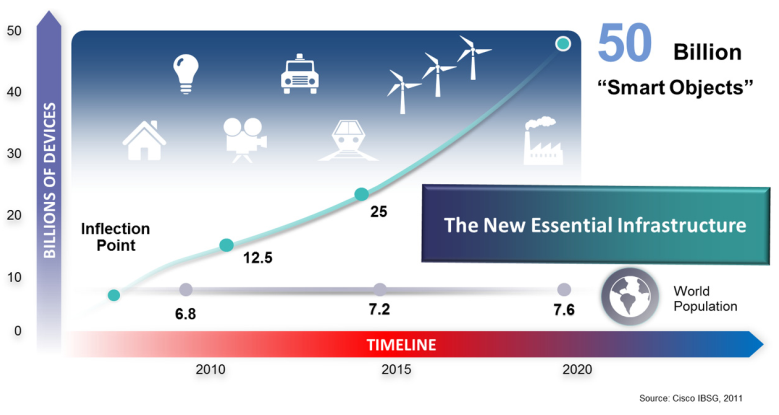
\includegraphics[scale = 0.5]{fig1.png}
	\caption{Các thiết bị kết nối Internet và sự phát triển trong tương lai}
	\label{fig:Graph1}
\end{figure}

Theo dự đoán, IoT sẽ là cơ sở hạ tầng cần thiết mới kết nối 50 tỷ thiết bị thông minh
trong năm 2020 khi dân số thế giới sẽ đạt mức 7.6 tỷ người. Được đề xuất bời liên
minh viễn thông quốc tế ITU, thì cơ sở hạ tầng này sẽ được xây dựng dựa trên kiến
trúc đa tầng nơi các thiết bị thông minh được sử dụng để cung cấp các dịch vụ khác
nhau. Dễ dàng nhận thấy, Internet nhúng không dây (Wireless Embedded Internet)
là một trong bốn thành phần quan trọng của một hệ thống IoT. Internet nhúng
không dây bao gồm các thiết bị nhúng giới hạn về tài nguyên, thường được cung
cấp điện năng bằng pin, và kết nối bởi các mạng không dây băng thông thấp, công
suất thấp tới Internet. Tuy nhiên, hiện nay có rất nhiều công nghệ vô tuyến độc quyền riêng được sử dụng
trong mạng IoT như: 802.15.4, Zigbee, Wi-fi, Bluetooth 4.0 Low Energy, NFC,
3GPP… dẫn đến trở ngại trong việc tích hợp với các mạng lớn hơn và với các dịch vụ trên nền Internet. \\

Để tiếp cận và bắt kịp các xu hướng trên, với sự hướng dẫn, tư vấn và định hướng của
thầy Võ Quế Sơn - giảng viên Bộ môn Viễn thông, em quyết định khai triển đề tài về Wireless
Sensor Networks dựa trên công nghệ 6LoWPAN/IPv6 và giao thức MQTT trên phần cứng là SoC TI
CC2538. Đề tài này tập trung nghiên cứu công nghệ 6LoWPAN và các ứng dụng trên đó được đề xuất để thiết kế một mô hình Wireless Sensor Networks giúp cho người dùng theo dõi dữ liệu từ cảm biến về nhiệt độ, nhịp tim, huyết áp và nồng độ oxy trong máu từ xa một cách dễ dàng.

\section{Nhiệm vụ luận văn}
\subsection{Mục đích của luận văn}
Mục đích của luận văn là nghiên cứu và cài đặt ứng dụng IoT dựa trên các công
nghệ mở rộng mới như IPv6, 6LoWPAN và IEEE 802.15.4
trên nền tảng hệ điều hành Contiki cho các thiết bị IoT. Từ đó có thể đưa vào sử
dụng thực tế các ứng dụng IoT đang là một hướng đi mới cho các doanh nghiệp
công nghệ thông tin và truyền thông hiện nay.
\subsection{Nhiệm vụ của đề tài}
Nhiêm vụ của luận văn là xây dựng hệ thống Wireless Sensor Network, thu thập dữ liệu y sinh từ
Board E-Health về cho người dùng thông qua mạng không dây sử dụng mạng 6LoWPAN/IPv6 và giao thức MQTT được chia thành các nhiệm vụ nhỏ sau: \\
\begin{itemize}
\item Nắm rõ các giao thức sếp ngăn được phát triển trong hệ điều hành Contik OS, đặc biệt là giao thức của 6LoWPAN/IPv6 được tích hợp trong lớp Network của Contiki OS. 
\item Nghiên cứu và thiết kế phần mềm cho các thiết bị phần cứng của hệ thống bao gồm board phát triển, board cảm biến, border-router. 
\item Kiểm tra, thử nghiệm phần cứng và phần mềm đã xây dựng thông qua việc kiểm tra hoạt động của mạch phần cứng cũng như kiểm tra các tính năng truyền nhận dữ liệu. 
\item Nghiên cứu phát triển phần mềm Android cho việc tương tác với người dùng dựa trên Flutter. 
\end{itemize}
\subsection{Nội dung thực hiện}
Các nội dung cần thực hiện để hoàn thành đề tài luận văn bao gồm các công việc sau:
\begin{itemize}
\item \textbf{Nội dung 1: Tìm hiểu lý thuyết mạng cảm biến không dây, cấu trúc và các ứng
dụng xung quanh:} Tìm hiểu về mạng cảm biến không dây, các chuẩn giao tiếp chính hiện
nay, mô hình mạng và các ứng dụng hiện nay để có cái nhìn tổng quan để tiến hành đề tài này.
\item \textbf{Nội dung 2: Nghiên cứu Contiki OS bao gồm các lớp trong ngăn xếp Contiki,
các chuẩn giao thức của mạng cảm biến:} Contiki OS bao gồm các giao thức và ngăn
xếp/ lớp khác nhau theo mô hình OSI, trong đó nổi bật là 6LoWPAN/IPv6, tìm hiểu về giao thức MQTT ứng dụng cho đề tài luận văn.
\item \textbf{Nội dung 3: Tìm hiểu phần cứng liên quan tới đề tài luận văn, đặc điểm, tính năng, chuẩn giao tiếp:} Ở nội dung này, sẽ tìm hiểu về Board E-Health, thu phát RF trong mạng 6LoWPAN/IPv6, các thông số cần thiết của phần cứng.
\item \textbf{Nội dung 4: Nghiên cứu và phát triển phần mềm cho đề tài:} Từ việc tìm hiểu Contiki OS
tích hợp 6LoWPAN/IPv6, từ đó lập trình cho việc truyền nhận RF cũng như giao tiếp với Board E-Health trong đề tài luận văn.
\item \textbf{Nội dung 5: Kiểm tra, thử nghiệm phần cứng thông qua việc test
các tính năng truyền nhận dữ liệu:} Việc kiểm tra phần cứng là một nhiệm vụ tất yếu, thông qua các bài test về udp-rpl, udp-border-router, test khả năng ổn định của board. Từ đây để chắc chắn một điều rằng, ít nhất phần cứng phải hoạt động để triển khai các nội dung khác.
\item \textbf{Nội dung 6: Nghiên cứu phát triển phần mềm Android cho việc tương tác với người
dùng bằng Flutter.}
\item \textbf{Nội dung 7: Tiến hành liên kết các phần: phần cứng, phần mềm để
đưa ra một hệ thống hoàn chỉnh. Đo đạc các thông số:} Sau khi đã thiết kế phần cứng, phần mềm thì việc tổng hợp liên kết chúng lại với nhau là điều tất yếu, từ đây sẽ đánh giá và cải thiện toàn bộ hệ thống trước khi đưa ra một hệ thống hoàn chỉnh hoàn toàn.
\item \textbf{Nội dung 8: Viết báo cáo, chuẩn bị slide thuyết trình:} Hoàn thành báo cáo đề tài
luận văn, slide thuyết trình và chuẩn bị cho phần bảo về đề tài.
\end{itemize}

\textbf{Bảng phân bố thời gian trong quá trình thực hiện đề tài:} 
\begin{table}[h]
\centering
\caption{Bảng phân bố thời gian trong quá trình thực hiện đề tài.}
\label{tab:tb1}
\begin{tabular}{|c|c|c|c|c|c|}
	\hline
	& \textbf{Tháng 1} & \textbf{Tháng 2} & \textbf{Tháng 3} & \textbf{Tháng 4} & \textbf{Tháng 5} \\ \hline
	Nội dung 1 & x                &                  &                  &                  &                  \\ \hline
	Nội dung 2 &                  & x                &                  &                  &                  \\ \hline
	Nội dung 3 &                  &                  & x                &                  &                  \\ \hline
	Nội dung 4 &                  &                  & x                &                  &                  \\ \hline
	Nội dung 5 &                  &                  & x                &                  &                  \\ \hline
	Nội dung 6 &                  &                  &                  & x                &                  \\ \hline
	Nội dung 7 &                  &                  &                  & x                &                  \\ \hline
	Nội dung 8 &                  &                  &                  &                  & x                \\ \hline
\end{tabular}
\end{table}
%%%%%%%%%%%%%%%%%%%%%%%%%%%%%%%%%
\newpage
\chapter{Lý thuyết}
\noindent
Ở chương 2 - Cơ sở lý thuyết, trình bày về lý thuyết của mạng cảm biến không dây cũng như
giới thiệu về Contiki OS, các ngăn xếp giao thức trong Contiki OS, từ đó giới thiệu về
6LoWPAN trên nền tảng hệ điều hành cho các thiết bị IoT này.
\section{Tổng quan về mạng cảm biến không dây}
\subsection{Giới thiệu mạng cảm biến không dây}
Một mạng cảm biến không dây là một mạng bao gồm nhiều nút cảm biến nhỏ có giá thành
thấp, và tiêu thụ năng lượng ít, giao tiếp thông qua các kết nối không dây, có nhiệm vụ cảm
nhận, đo đạc, tính toán nhằm mục dích thu thập, tập trung đữ liệu để đưa ra các quyết định
toàn cục về môi trường từ cảm biến. \\

\noindent
\textbf{Nút cảm biến bao gồm:} vi điều khiển (microcontroller), bộ truyền nhận (transceiver), bộ nhớ (memory), nguồn cung cấp (power source) và các cảm biến.
(sensors).
\begin{itemize}
\item Microcontroller: thực hiện các nhiệm vụ, xử lí dữ liệu và điều khiển các thành phần khác
trong nút cảm biến. Một microcontroller thường sử dụng nhiều hệ thống nhúng như các sensor,
có khả năng kết nối với các phần cứng khác, dễ dàng lập trình và sử dụng năng lượng thấp.
\item Transceiver: giao tiếp thông dụng nhất là RF vì khả năng tích hợp trong mạng WSN:. Trong
WSN, các băng tần thường được sử dụng như 173, 433, 868, 915 MHz và 2.4GHz. Và cũng có
nghĩa là nó vừa có khả năng truyền cũng như nhận tín hiệu.
\item Memory: hầu hết các Microcontroller đều có tích hợp sẵn Flash Memory, RAM, ROM. Tùy
theo từng loại microcontroller mà dung lượng của các vùng nhớ này sẽ tương ứng theo đó.
Ngoài ra cũng có thể sử dụng các bộ nhớ ngoài cho chúng, tăng vùng nhớ tới dung lượng mong
muốn.
\item Power Source: tùy theo loại ứng dụng mà có thể sử dụng các nguồn cung cấp cho phù hợp,
đặt biệt với các ứng dụng có địa điểm thu thập khó tiếp cận thì việc sử dụng pin trở nên bắt
buộc, từ đó việc quản lý nguồn cũng là một trong những vẫn đề quan trọng. Khi nghiên cứu về mạng cảm biến không dây, một trong những đặc điểm quan trọng và then chốt là thời gian sống của các cảm biến hay chính là sự giới hạn về năng lượng của chúng. Các nút cảm biến hoạt động có thời hạn và không thể thay thế được nguồn cung cấp. Do đó, trong khi mạng truyền thông tập trung vào các dịch vụ chất lượng cao, thì các giao thức mạng cảm biến phải tập trung vào bảo toàn công suất.
\item Sensors: Sensors được sử dụng để có thể bắt dữ liệu từ môi trường quanh nó, sensors có thể
được tích hợp trên nút cảm biến hoặc giao tiếp với nút qua module ngoài. Sensors có thể giao
tiếp qua tin hiệu analog, từ đó chuyển thành tín hiệu số thông qua bộ ADC, hoặc có thể giao
tiếp qua tín hiệu số qua các chuẩn giao tiếp như I2C, SPI, UART,...
\end{itemize}
\begin{figure}[h]
	\centering
	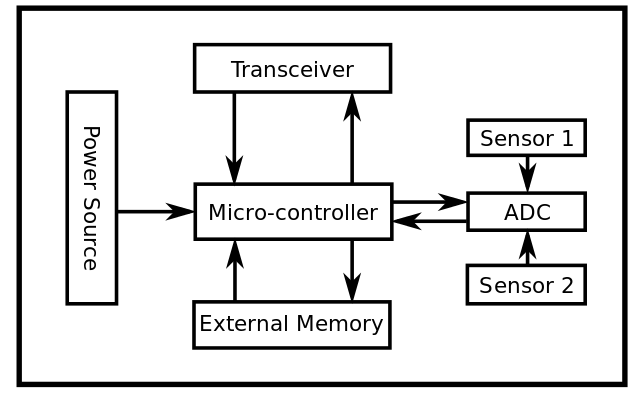
\includegraphics[scale = 0.3]{fig2.png}
	\caption{Cấu trúc nút cảm biến}
	\label{fig:Graph2}
\end{figure}
\textbf{Mạng cảm biến có một số đặc điểm sau:}
\begin{itemize}
\item Mạng không dây: các mạng liên lạc với nhau qua bộ thu phát không dây để trao đổi và xử lý dữ liệu được thu thập bởi bộ phận cảm biến của chúng. 
\item Có khả năng tự tổ chức, yêu cầu ít hoặc không có sự can thiệp của con người.
\item Truyền thông không tin cậy, phạm vi hoạt động hẹp, định tuyến multihop.
\item Triển khai dày đặc và khả năng kết hợp giữa các nút cảm biến.
\item Cấu hình mạng thay đổi thường xuyên phụ thuộc vào fading và hư hỏng ở các nút cảm
biến.
\item Năng lượng thấp: WSN có thể được lắp đặt ở những vị trí xa nơi không có sẵn nguồn điện. Để có thể hoạt động trong vài tháng trong nhiều năm, các nút phải sử dụng bộ vi xử lý và bộ thu phát không dây công suất thấp và thực hiện các kế hoạch tiết kiệm điện. Bộ xử lý phải chuyển sang chế độ ngủ càng lâu càng tốt và lớp Medium-Access phải được thiết kế phù hợp. 
\end{itemize}
\newpage
\subsection{Cấu trúc mạng cảm biến không dây}
Cấu trúc mạng cảm biến bao gồm các nút cảm biến, trường cảm biến, internet và người dùng được thể hiện trong hình bên dưới.
\begin{figure}[h]
	\centering
	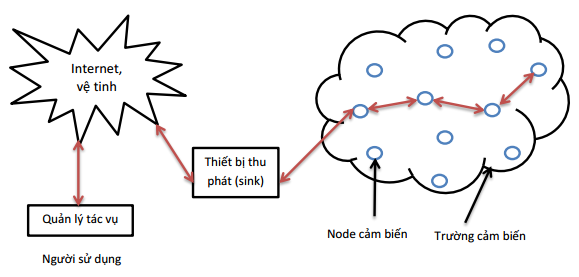
\includegraphics[scale = 0.7]{fig3.png}
	\caption{Cấu trúc mạng cảm biến không dây}
	\label{fig:Graph3}
\end{figure}

Đối với mạng cảm biến, các node cảm biến được phân bố trong môi trường với mật độ đủ để quan sát được các thay đổi của môi trường và đồng thời đảm bảo được việc thông báo cho người giám sát biết sự thay đổi ấy khi cần. Các node giao tiếp không dây qua sóng RF, do đó bị ảnh hưởng và hạn chế bởi vật cản hay khoảng cách. Khi muốn truyền đi xa thì các nút này phải phát với công suất lớn, khi đó mặt năng lượng có thể không được đảm bảo. Do đó để giảm công suất thì cần dùng giao tiếp multihop giữa các node. \\

Các nút trong mạng cảm biến hoạt động trong hầu hết các tình huống. Một mạng có thể bao gồm hàng trăm hoặc hàng nghìn nút, tùy thuộc vào ứng dụng. Mỗi nút cảm biến có khả năng thu thập dữ liệu và định tuyến trở lại thông qua thiết bị thu phát (sink) đến người dùng cuối theo kiến trúc Multi-hop infrastructure-less. Thiết bị thu phát (sink) sẽ liên lạc với nút quản lý tác vụ thông qua internet và vệ tinh. Để đạt được tuổi thọ mạng cao hơn, các nút cảm biến phải điều chỉnh các hoạt động của chúng theo cách hiệu quả về mặt năng lượng. Mỗi nút cảm biến sử dụng ngăn xếp giao thức để giao tiếp với các nút khác và thiết bị thu phát (sink). Về giao tiếp và làm việc hiệu quả trên nhiều nút cảm biến, ngăn xếp giao thức phải hoạt động hiệu quả về mặt năng lượng. \\

\noindent
\textbf{Đặc điểm của cấuu trúc mạng cảm biến không dây} \\
\indent
Mạng cảm biến không dây bao gồm một số lượng lớn các nút cảm biến, các nút cảm biến có
giới hạn và ràng buộc về tài nguyên. Do đó, cấu trúc mạng mới có đặc điểm rất khác với mạng
truyền thống, sau đây là một số phân tích một số đặc điểm nổi bật trong mạng cảm biến như
Sau:
\begin{itemize}
\item Khả năng chịu lỗi: Một số các nút cảm biến có thể không hoạt động nữa do thiếu năng lượng,
do những hư hỏng vật lý hoặc do ảnh hưởng của môi trường. Khả năng chịu lỗi thể hiện ở việc
mạng vẫn hoạt động bình thường, duy trì những chức năng của nó ngay cả khi một số nút
mạng không hoạt động.
\item Khả năng mở rộng: Khi nghiên cứu một số hiện tượng, số lượng các nút cảm biến được triển
khai có thể đến hàng trăm, hàng ngàn nút, phụ thuộc vào từng ứng dụng, con số này còn có
thể nhiều hơn. Do đó, cấu trúc mạng mới phải có khả năng mở rộng để có thể làm việc với số
lượng lớn các nút.
\item Giá thành sẵn xuất: Vì các mạng cảm biến bao gồm một số lượng lớn các nút cảm biến nên
chi phí của mỗi nút rất quan trọng trong việc khai triển chi phí cho toàn mạng. Do đó, chi phí
của mỗi nút cảm biến phải giữ ở mức thấp.
\item Ràng buộc phần cứng: Kích thước phải nhỏ, tiêu thụ năng lượng thấp, có khả năng hoạt
động ở những nơi có mật độ cao, chi phí sản xuất thấp, có khả năng tự trị và hoạt động không
cần sự giám sát của con người, thích nghi với môi trường.
\item Môi trường hoạt động: Các nút cảm biến được thiết lập dày đặc, rất gần hoặc trực tiếp bên
trong các hiện tượng để quan sát. Vì thế, chúng thường làm việc mà không cần giám sát, chúng
có thể làm việc trong các máy móc lớn, dưới dáy biển, những vùng ô nhiễm, khí độc, những
vùng xa xôi, hiểm trở hoặc các tòa nhà, cao ốc, hộ gia đình.
\item Phương tiện truyền dẫn: Ỏ những mạng cảm biến, các nút được kết nối bằng những phương
tiện không dây. Các kết nối này có thể tạo nên bởi sóng vô tuyến, hồng ngoại hoặc những
phương tiện quang học. Để thiết lập sự hoạt động thống nhất của mạng, các phương tiện
truyền dẫn phải theo chuẩn đã được công nhận trên toàn thế giới. Hiện tại nhiều phần cứng
của các nút cảm biến đều sử dụng RF làm phương tiện truyền thông không dây.
\item Sự tiêu thụ năng lượng: Trong một số ứng dụng, việc bổ sung năng lượng không thể thực
hiện được. Vì thế thời gian sống của các nút cảm biên phụ thuộc vào thời gian sống của pin.
Ở mạng cảm biến ad-hoc, mỗi một nút đóng một vai trò kép vừa khởi tạo vừa định tuyến nên
sự trục trặc của một nút cảm biến có thể gây ra những thay đổi đáng kể trong cấu hình và yêu
cầu định tuyến lại các gói tin và tổ chức lại mạng. Vì vậy việc duy trì và quản lý nguồn năng
lượng đóng vai trò quan trọng.
\end{itemize}

\noindent
\textbf{Kiến trúc giao thức mạng} \\
\begin{figure}[h]
	\centering
	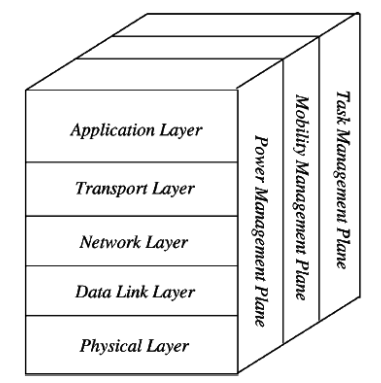
\includegraphics[scale = 0.7]{fig4.png}
	\caption{Kiến trúc giao thức mạng cảm biến.}
	\label{fig:Graph4}
\end{figure}

\indent
Kiến trúc giao thức này phối hợp các tính toán về định tuyến và năng lượng, kết hợp số liệu
với các giao thức mạng, truyền tin với hiệu quả về năng lượng thông qua môi trường không
dây và tăng cường sự hợp tác giữa các nút cảm biến. Kiến trúc giao thức bao gồm lớp ứng
dụng (Application Layer), lớp giao vận (Transport Layer), lớp mạng (Network Layer), lớp liên
kết số liệu (Datalink Layer), lớp vật lý (Physical Layer), mặt bằng quản lý năng lượng (Power
Management Plane), mặt bằng quản lý di động (Mobility Management Plane) và mặt bằng
quản lý nhiệm vụ (Task Management Plane). 
\begin{itemize}
\item Lớp ứng dụng: Vai trò của lớp ứng dụng là tóm tắt cấu trúc liên kết vật lý của mạng cảm biến không dây (WSN) ở dạng dữ liệu có thể đọc được cho các ứng dụng. Hơn nữa, lớp ứng dụng cung cấp các giao diện cần thiết để người dùng tương tác với thế giới vật lý thông qua WSN.
\item Lớp truyền tải: Một lớp truyền tải là cần thiết trong các mạng cảm biến không dây để kiểm soát tắc nghẽn và đảm bảo gửi thông điệp đáng tin cậy từ các nút cảm biến đến nút sink. Năng lượng hạn chế, bộ nhớ và tài nguyên tính toán của các nút cảm biến yêu cầu một lớp vận chuyển hiệu quả năng lượng.
\item Lớp mạng: Chức năng chính của lớp này là định tuyến; nó xử lý việc định tuyến dữ liệu trên toàn mạng từ điểm nguồn đến điểm đích. Bằng cách đáp ứng các ràng buộc của giao thức như năng lượng hạn chế, băng thông truyền thông, bộ nhớ và khả năng tiêu thụ có thể kéo dài tuổi thọ của mạng. Định tuyến tiết kiệm năng lượng, định tuyến tập trung dữ liệu và tổng hợp dữ liệu là một số nhiệm vụ quan trọng được thực hiện bởi lớp mạng cung cấp kết nối internet với các mạng bên ngoài như internet và các hệ thống chỉ huy và điều khiển. Hầu hết dữ liệu trong mạng cảm biến sẽ được hướng về nút sink. Các giao thức định tuyến đa bước đặc biệt là cần thiết giữa các nút sink và nút cảm biến cho mạng cảm biến không dây.
\item Lớp liên kết dữ liệu: Chịu trách nhiệm ghép kênh các luồng dữ liệu, phát hiện khung dữ liệu, truy cập phương tiện, kiểm soát lỗi và MAC. Nó đảm bảo các kết nối điểm-điểm và điểm-đa điểm đáng tin cậy trong mạng truyền thông. Giao thức MAC trong mạng cảm biến tự tổ chức multihop không dây cần đạt được hai mục tiêu. Đầu tiên là việc tạo ra cơ sở hạ tầng mạng. Vì hàng nghìn nút cảm biến nằm rải rác dày đặc trong một trường cảm biến, MAC phải thiết lập các liên kết truyền thông để truyền dữ liệu. Điều này tạo thành cơ sở hạ tầng cơ bản cần thiết cho giao tiếp không dây và mang lại cho mạng cảm biến khả năng tự tổ chức. Mục tiêu thứ hai là chia sẻ công bằng và hiệu quả tài nguyên giao tiếp giữa các nút cảm biến. Vì môi trường ồn ào và các nút cảm biến có thể di động, giao thức MAC phải nhận biết được nguồn điện và có thể giảm thiểu va chạm với các chương trình phát sóng của hàng xóm.
\item Lớp vật lý: Các chức năng chính của lớp vật lý là lựa chọn và tạo tần số sóng mang, mã hóa và giải mã, điều chế và giải điều chế, truyền và nhận dữ liệu. Mạng cảm biến không dây thường hoạt động trong các băng tần ISM.
\item Kế hoạch quản lý nguồn: Cách một nút cảm biến sử dụng nguồn của nó được quản lý bởi kế hoạch quản lý nguồn. Nếu mức công suất cảm biến ở mức thấp, nó sẽ ngừng tham gia vào quá trình định tuyến và thông báo trạng thái công suất thấp cho hàng xóm. Để nhận được các tin nhắn trùng lặp, nút cảm biến có thể tắt tính năng nhận tin nhắn từ những người hàng xóm.
\item Kế hoạch quản lý tính di động: Các chuyển động của các nút cảm biến được đăng ký và phát hiện bởi kế hoạch quản lý tính di động. Kết quả lộ trình quay trở lại người dùng được duy trì. Vì vậy, nút cảm biến có thể duy trì các bản ghi cân bằng giữa việc sử dụng tác vụ và năng lượng của chúng.
\item Kế hoạch quản lý nhiệm vụ: Nó cân bằng và lên lịch các nhiệm vụ cảm biến cho một khu vực cụ thể. Kế hoạch quản lý tác vụ này là bắt buộc đối với dữ liệu định tuyến trong mạng cảm biến di động, nút cảm biến có thể hoạt động cùng nhau theo cách hiệu quả về năng lượng và chia sẻ tài nguyên giữa các nút cảm biến.
\end{itemize}
\subsection{Ứng dụng của mạng cảm biến không dây}
Mạng cảm biến không dây được ứng dụng đầu tiên trong các lĩnh vực quân sự. Cùng với
sự phát triển của ngành công nghiệp tự động, robotic, thiết bị thông minh, môi trường, y tế,
nông nghiệp... mạng cảm biến không dây ngày càng được sử dụng nhiều trong hoạt động công
nghiệp và dân dụng.
\begin{figure}[h]
	\centering
	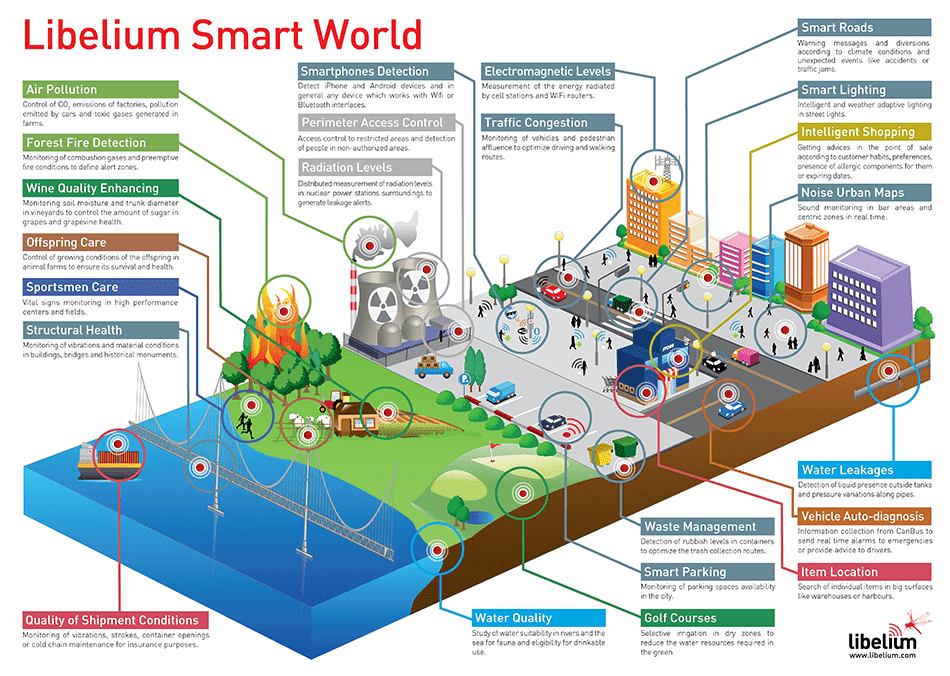
\includegraphics[scale = 0.5]{fig5.png}
	\caption{Ứng dụng của mạng cảm biến không dây}
	\label{fig:Graph5}
\end{figure}\\
\newpage
\noindent
\textbf{Một số ứng dụng cơ bản của mạng cảm biến không dây:} \\

\indent
Cảm biến môi trường: Các mạng cảm biến không dây được dùng để theo đõi sự chuyển động
của chim, động vật, côn trùng; theo dõi các điều kiện môi trường như nhiệt độ, độ ẩm;
theo dõi và cảnh báo sớm các hiện tượng thiên tai như động đất,núi lửa phun trào, cháy rừng,
lũ lụt... Một số ứng dụng quan trọng như: Phát hiện sớm những thảm họa như cháy rừng, Cảnh báo lũ lụt, Giám sát và cảnh báo các hiện tượng địa chấn...
\begin{figure}[h]
	\centering
	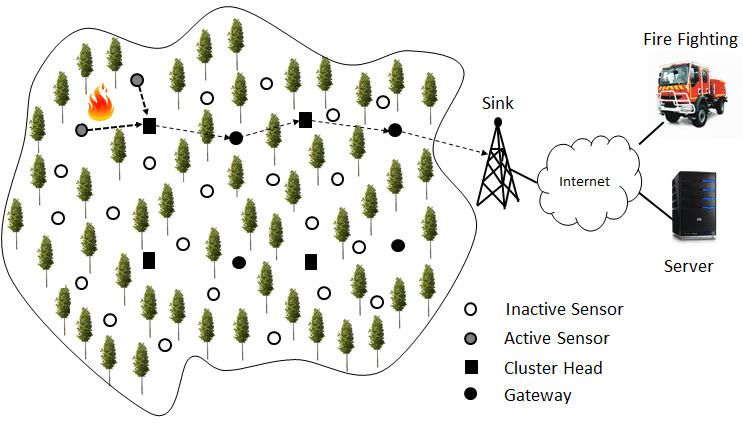
\includegraphics[scale = 0.5]{fig6.png}
	\caption{Mạng cảm biến không dây báo cháy rừng}
	\label{fig:Graph6}
\end{figure}\\

Các ứng dụng trong y học: Giám sát trong y tế và chẩn đoán từ xa. Trong tương lai, các nút
cảm ứng có thể được gắn vào cơ thể, ví dụ như ở dưới da và đo các thông số của máu để phát
hiện sớm các bệnh như ung thư, nhờ đó việc chữa bệnh sẽ dễ dàng hơn. Hiện nay đã tồn tại
những cảm biến rất nhỏ có thể nuốt vào trong người, dùng một lần và được bọc vỏ hoàn toàn,
nguồn nuôi của thiết bị này đủ để hoạt động trong 24h. Trong thời gian đó, chúng
gửi hình ảnh về bên trong con người sang một thiết bị khác mà không cần phải phẫu thuật.
Các bác sĩ có thể dựa vào đó để chuẩn đoán và điều trị.
%\newpage
\begin{figure}[h]
	\centering
	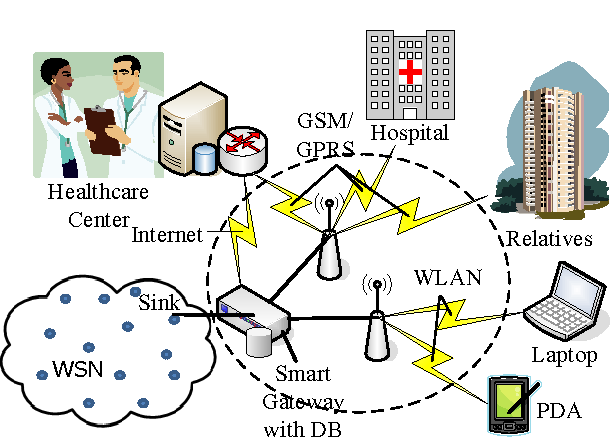
\includegraphics[scale = 0.4]{fig7.png}
	\caption{Mạng cảm biến không dây trong y tế}
	\label{fig:Graph7}
\end{figure}
\newpage
Ứng dụng trong gia đình: Trong căn nhà thông minh, các đồ dùng và thiết bị điện trong nhà từ phòng ngủ, phòng khách đến toilet đều có thể gắn các bộ điều khiển điện tử có thể kết nối với Internet và điện thoại di động, cho phép chủ nhân điều khiển vật dụng từ xa hoặc lập trình cho thiết bị ở nhà hoạt động theo lịch. Thêm vào đó, các đồ gia dụng có thể hiểu được ngôn ngữ của nhau và có khả năng tương tác với nhau.
\begin{figure}[h]
	\centering
	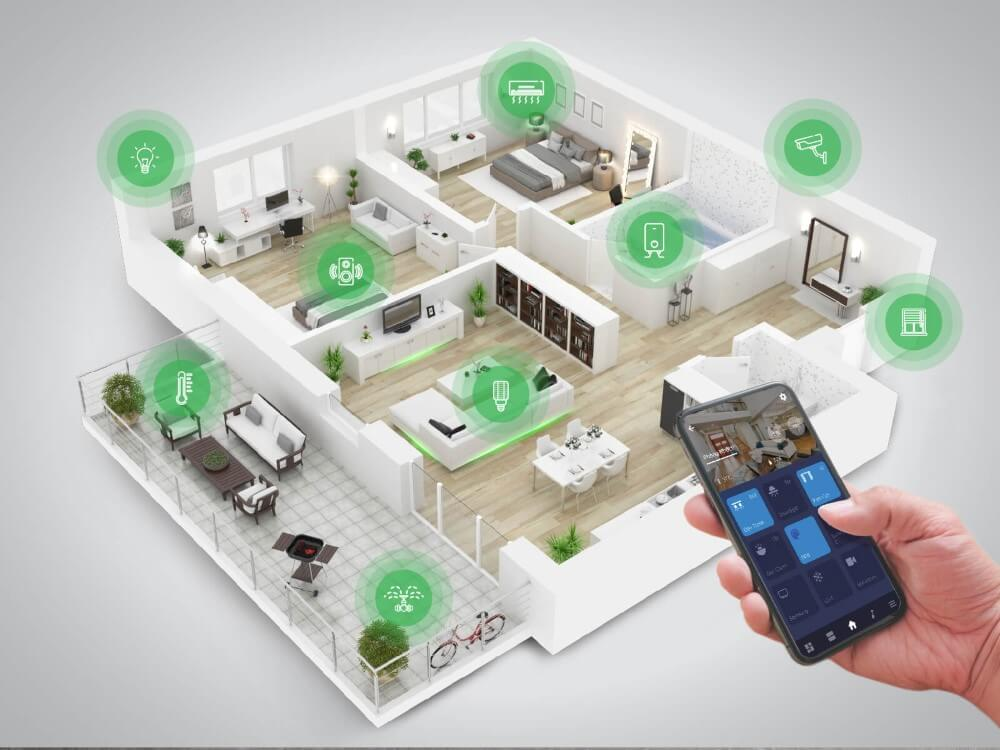
\includegraphics[scale = 0.3]{fig8.png}
	\caption{Mạng cảm biến không dây trong nhà thông minh}
	\label{fig:Graph8}
\end{figure}\\

Ứng dụng trong công nghiệp
\begin{itemize}
\item Trong lĩnh vực quản lý kinh doanh là bảo quản và lưu giữ hàng hóa.
\item Trong việc quản lý các container ở cảng. Mỗi một container là một nút mạng trong mạng cảm ứng và có thể ghi nhớ thông tin của nó một cách xác thực. Việc liên lạc qua khoảng cách xa hơn có thể thực hiện theo kiểu điểm — điểm từ container này đến container khác. Tập hợp các container tự bản thân nó là một cơ sở dữ liệu và vì vậy luôn luôn nhất quán. Nhờ đó tàu có thể dễ dàng xác định được chính xác kiện hàng của nó và container thậm chí còn có thể thông báo lại nếu có container lân cận bị lỡ, mà không cần phải truy nhập vào đữ liệu toàn cục (global database).
\item Quản lí dây truyền sản xuất, theo dõi sản phẩm: Các nút cảm biến tích hợp trong các
thiết bị trong sản xuất sản phẩm giúp cho việc giám sát, kiểm tra, báo cáo tất cả các hoạt
động sản xuất. Các thiết bị có thể giao tiếp với nhau, làm thông tin của nhau. Ứng dụng cảm
biến vào sản xuất này sẽ giúp tăng năng suất, tăng tính tự động hóa, tăng độ tin cậy cho sản
phẩm, tạo ra những sản phẩm chất lượng, năng suất sản xuất hiệu quả.
\end{itemize}
\newpage
Ứng dụng trong nông nghiệp
\begin{itemize}
\item Ứng dụng trong trồng trọt: Các cảm biến được dùng để do nhiệt độ, độ ẩm, ánh sáng ở
nhiều điểm trên thửa ruộng và truyền dữ liệu mà chúng thu được về trung tâm để người nông
dân có thể giám sát và chăm sóc, điều chỉnh cho phù hợp.
\end{itemize}
\begin{figure}[h]
	\centering
	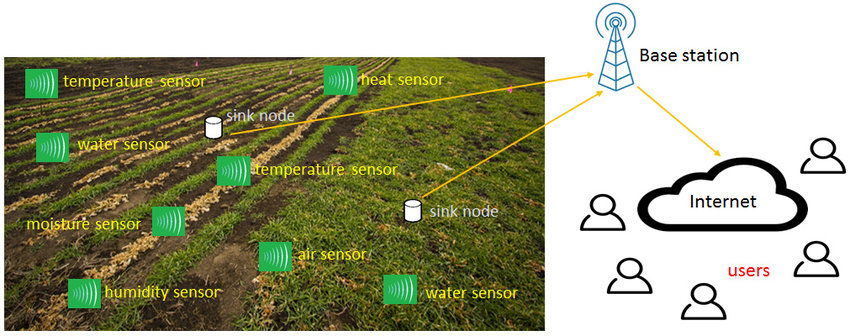
\includegraphics[scale = 0.5]{fig9.png}
	\caption{Mạng cảm biến không dây trong trồng trọt}
	\label{fig:Graph9}
\end{figure}
\begin{itemize}
\item Ứng dụng trong chăn nuôi: Trong chăn nuôi gia súc, gia cầm cũng trang bị các cảm biến
để dễ dàng theo dõi và giám sát.
\end{itemize}
\begin{figure}[h]
	\centering
	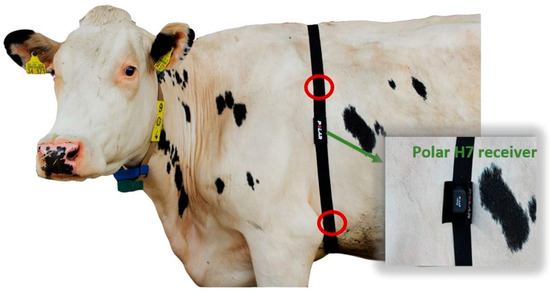
\includegraphics[scale = 0.5]{fig10.png}
	\caption{Mạng cảm biến không dây trong chăn nuôi}
	\label{fig:Graph10}
\end{figure}

Ứng dụng trong quân sự: Có tiềm năng rất lớn cho các mạng cảm biến không dây trong các lĩnh vực an ninh và giám sát. Trong các ứng dụng quân sự, motes chủ yếu được sử dụng trong giám sát biên giới, theo dõi và phân loại các hoạt động của đối phương. Một trong những ứng dụng quan trọng của motes là phát hiện chuyển động bằng cách sử dụng cảm biến khoảng cách có thể được sử dụng để giám sát các mỏ đất được coi là nguy hiểm đối với con người khi tiếp cận. Hiện tại, máy bay không người lái chiến đấu được dùng rất phổ biến trong việc tấn công căn cứ của đối phương mà không có phi công trên máy bay và sự điều khiển của con người trong thời gian thực giúp giảm thiệt hại về nhân mạng. Các ứng dụng WSN cũng có thể được sử dụng trong các hoạt động thường xuyên như an ninh nội địa, tuần tra biên giới, bảo vệ tài sản, v.v.
\newpage
\begin{figure}[h]
	\centering
	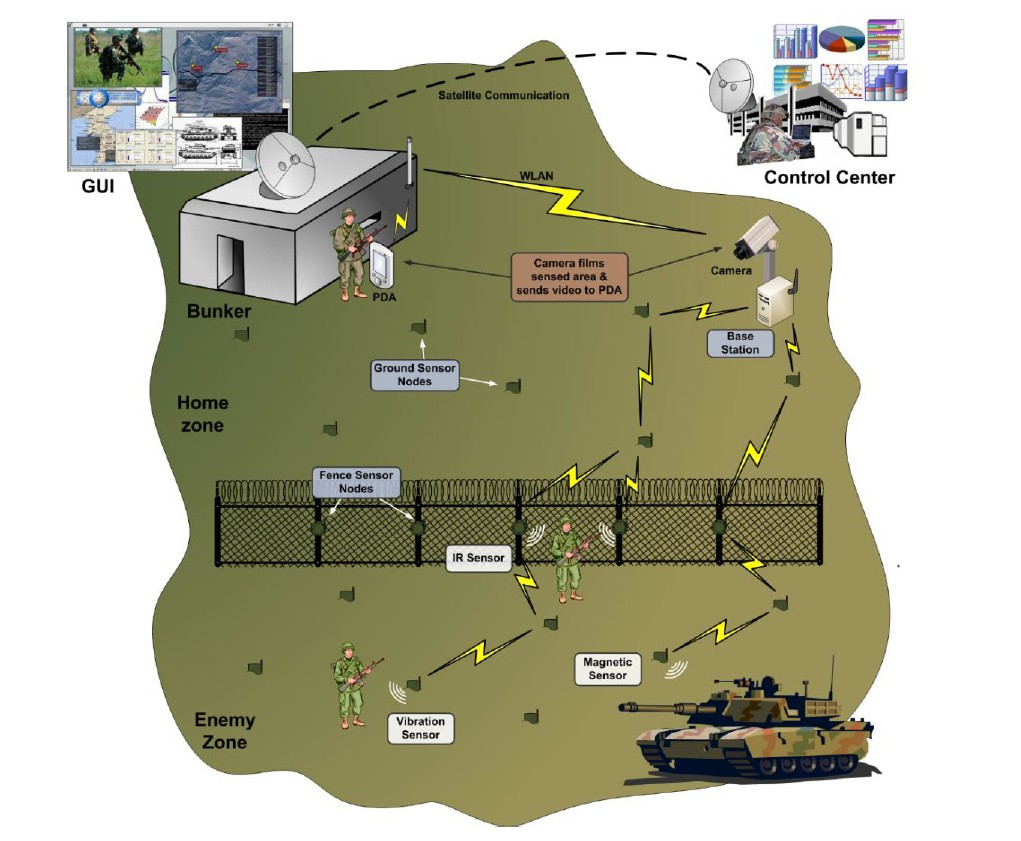
\includegraphics[scale = 0.5]{fig11.png}
	\caption{Mạng cảm biến không dây trong quân sự}
	\label{fig:Graph11}
\end{figure}

Trong giao thông: Các ứng dụng phát hiện giao thông điển hình như phát hiện lấn làn và đo tốc độ của phương tiện giao thông. Một cảm biến không dây được đặt ở giữa làn đường giao thông để phát hiện sự hiện diện và đi qua của phương tiện. Để đo tốc độ và chiều dài của xe, hai cảm biến không dây được căn chỉnh theo trục làn được lắp đặt như hình dưới.
\begin{figure}[h]
	\centering
	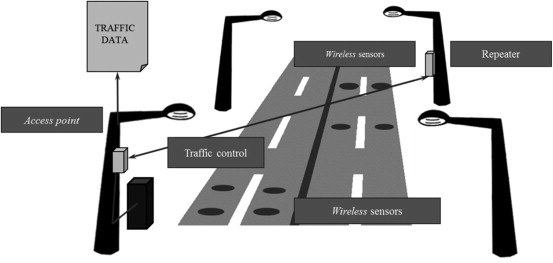
\includegraphics[scale = 0.5]{fig12.png}
	\caption{Mạng cảm biến không dây trong giao thông}
	\label{fig:Graph12}
\end{figure}
\newpage
\section{Contiki OS — Hệ điều hành mã nguồn mở cho IoT}
Contiki là một hệ điều hành nguồn mở, đa tác vụ, có tính linh động cao, phát triển
cho các mạng cảm biến không dây và các hệ thống nhúng kết nối mạng hiệu quả về
bộ nhớ, được thiết kế cho các bộ vi xử lý với một lượng bộ nhớ nhỏ. Contiki được phát triển bởi một nhóm các nhà phát triển từ các ngành công nghiệp và học viện do Adam Dunkels từ Viện Khoa Học Máy Tính Thụy Điển dẫn đầu. Nhóm Contiki hiện bao gồm mười sáu nhà phát triển từ SICS, SAP AG, Cisco, Atmel, NewAE và TU Munich. \\

Contiki được thiết kế cho các hệ thống nhúng với một lượng nhỏ bộ nhớ. Một cấu hình điển
hình Contiki là 2 kilobyte bộ nhớ RAM và 40 kilobytes ROM. Contiki bao gồm một hạt nhân
event-driven ở lớp trên của chương trình ứng dụng. Contiki sử dụng protothreads cung cấp một
phong cách lập trình tuyến tính. Contiki cũng hỗ trợ cho mỗi quá trình tùy chọn ưu tiên đa
luồng, interprocess giao tiếp bằng cách sử dụng thông qua các gói tin sự kiện, cũng như một
tùy chọn giao diện hệ thống với hỗ trợ trực tiếp cho các thiết bị đầu cuối kết nối tại local hoặc
nối mạng ảo hiển thị với VNC hoặc qua Telnet. \\ 

Contiki cung cấp kết nối Internet tiêu thụ điện năng thấp, nó cũng hỗ trợ giao tiếp
IP, cả IPv4 và IPv6, cùng với các chuẩn không dây công suất thấp gần đây như:
6lowpan, RPL, CoAP, MQTT. Với ContikiMAC và sleepy routers, các bộ định
tuyến không dây thậm chí có thể hoạt động bằng pin. \\

Contiki chứa hai ngăn xếp giao tiếp: uIP và Rime. uIP là một ngăn xếp TCP / IP nhỏ tuân thủ RFC giúp Contiki có thể giao tiếp qua Internet. Rime là một ngăn xếp liên lạc nhẹ được thiết kế cho bộ đàm công suất thấp. Rime cung cấp một loạt các nguyên tắc giao tiếp, từ phát sóng khu vực cục bộ với nỗ lực tốt nhất, cho đến việc cung cấp dữ liệu số lượng lớn đa bước nhảy đáng tin cậy. \\

Contiki chạy trên nhiều nền tảng khác nhau, từ các bộ vi điều khiển nhúng như MSP430 và AVR đến các máy tính. Contiki được viết bằng ngôn ngữ lập trình C và được cung cấp miễn phí dưới dạng mã nguồn mở theo giấy phép kiểu BSD.
\begin{figure}[h]
	\centering
	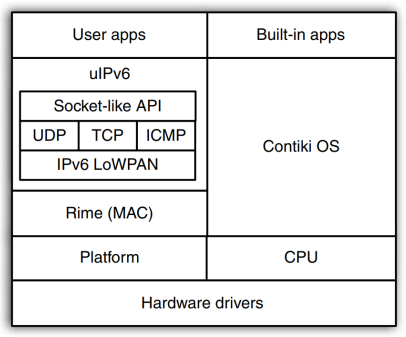
\includegraphics[scale = 0.4]{fig13.png}
	\caption{Ngăn xếp trong Contiki}
	\label{fig:Graph13}
\end{figure}
Contiki OS hỗ trợ các giao thức chuẩn IETF cho mạng IPv6 năng lượng thấp, bao gồm 6LoWPAN, giao thức multihop routing và một số giao thức ở lớp ứng dụng như CoAP, MQTT...
Các lớp giao thức được phân bố theo các stack, dựa vào đó Contiki OS đề xuất các tầng giao thức
như sau:
\begin{figure}[h]
	\centering
	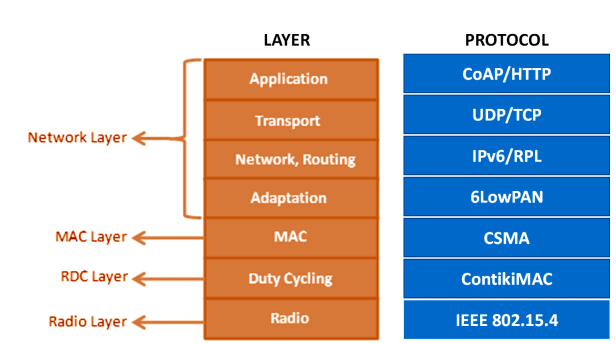
\includegraphics[scale = 0.6]{fig14.png}
	\caption{Các tầng giao thức trong Contiki}
	\label{fig:Graph14}
\end{figure}
\subsection{Application Layer}
Lớp ứng dụng chịu trách nhiệm định dạng dữ liệu. Nó cũng đảm bảo rằng dữ liệu được vận
chuyển trong các chương trình tối ưu ứng dụng. Trong đề tài luận văn này, ở lớp ứng dụng tôi sử dụng giao thức MQTT để giao tiếp với ứng dụng Android trên điện thoại. \\

\textbf{MQTT (Message Queuing Telemetry Transport)} \\

MQTT (Message Queuing Telemetry Transport) là một giao thức truyền thông điệp (mes-
sage) theo mô hình publish/subscribe, sử dụng băng thông thấp, độ tin cậy cao và có khả năng
hoạt động trong điều kiện đường truyền không ổn định. \\

MQTT được tạo ra từ năm 1999 bởi hai kỹ sư - Andy Stanford-Clark (IBM) và Arlen Nipper
(Eurotech) khi họ phải phát minh ra một giao thức mới để kết nối các đường ống dẫn dầu thông qua
các mạng vệ tinh không đáng tin cậy. Năm 2011, IBM và Eurotech đã tặng MQTT cho dự án
Eclipse được đề xuất có tên là Paho. Trong năm 2013, nó đã được đệ trình lên OASIS để chuẩn
hóa. \\

MQTT gồm 2 thành phần chính: 
\begin{itemize}
\item MQTT Broker: MQTT broker là một phần mềm chạy trên máy tính (chạy trực tiếp trên máy hoặc trên đám mây) và có thể được tự xây dựng hoặc host bởi bên thứ ba. Các phần mềm MQTT broker ngày nay có ở hai dạng mã nguồn mở và triển khai độc quyền. Các broker hoạt động như một bưu điện, MQTT không sử dụng địa chỉ của người sẽ được nhận tin nhắn mà sử dụng cơ chế quản lý theo "topic", và bất kỳ ai muốn có một bản sao của tin nhắn được gởi sẽ phải đăng ký topic đó. Nhiều client có thể nhận được tin nhắn từ một broker duy nhất. Tương tự, nhiều publisher có thể xuất bản (publish) các topic cho một người đăng ký.
\item Client: Được chia thành 2 nhóm là publisher và subscriber. Client là bất kỳ thiết bị nào (từ vi điều khiển đến một máy chủ chính thức) chạy thư viện MQTT và kết nối tới MQTT broker qua mạng. Client chỉ làm ít nhất một trong 2 việc là publish các message lên một topic cụ thể hoặc surscribe lên một topic nào đó để nhận message từ topic này.
\end{itemize}

Cách thức hoạt động: 
\begin{itemize}
\item MQTT quản lý các thông tin - dữ liệu mà nó nhận được theo hệ thống cấp bậc của các topic (tạm dịch: chủ đề). Với cơ chế publish-subscribe của MQTT, khi một publisher có một dữ liệu muốn truyền đi, nó sẽ gởi một tin nhắn điều khiển (control message) với dữ liệu muốn truyền đi đó đến MQTT broker mà nó đã kết nối đến. Broker sau đó sẽ gởi các thông tin mà nó nhận được này đến client đã đăng ký (subscribe) vào topic đó. Các publisher không cần có bất cứ thông tin nào về số lượng hay vị trí của các subscriber, đồng thời, các subscriber cũng không cần phải được cấu hình để có bất kì thông tin gì về các publisher.
\item Nếu một broker nhận một tin nhắn trên một topic mà hiện tại không có subscriber, broker sẽ bỏ tin nhắn đó đi, trừ khi publisher của tin nhắn đó chỉ định tin nhắn đó là một retained message (tạm dịch: tin nhắn được giữ lại). Một retained message là một tin nhắn MQTT thông thường với cờ retained được gán giá trị true. Broker lưu retained message cuối cùng và QoS tương ứng cho topic được chọn. Mỗi client đăng ký (subscribe) vào một topic phù hợp với topic của retained message sẽ ngay lập tức nhận được retained message đó sau khi client đó đăng ký. Broker chỉ lưu một retained message cho từng topic. Cơ chế này cho phép một subscriber mới của một topic có thể nhận được những thông tin mới nhất, hơn là phải chờ đợi lần cập nhật tiếp theo từ một publisher. Client chỉ tương tác với một broker, nhưng một hệ thống có thể chứa một số máy chủ làm broker với nhiệm vụ trao đổi dữ liệu dựa trên các topic hiện tại được các client đăng ký.
\end{itemize}
\begin{figure}[h]
	\centering
	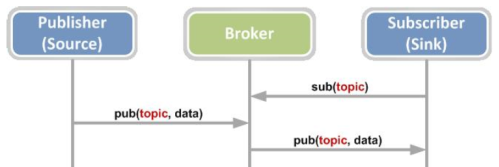
\includegraphics[scale = 0.7]{fig15.png}
	\caption{MQTT Publish-Subscribe}
	\label{fig:Graph15}
\end{figure}

MQTT định nghĩa ba mức chất lượng dịch vụ (QoS):
\begin{itemize}
\item QoS 0: trình môi giới/máy trạm sẽ phân phát tin nhắn một lần, và không có xác
nhận (gửi và lãng quên).
\item QoS 1: trình môi giới/máy trạm sẽ phân phát tin nhắn ít nhất một lần, có yêu cầu
xác nhận.
\item QoS 2: trình môi giới/máy trạm sẽ phân phát tin nhắn chính xác một lần bằng
cách sử dụng bắt tay bốn bước.
\end{itemize}
\newpage
Các tính năng khác của MQTT là:
\begin{itemize}
\item Các bản tin keep-alive (PINGREQ, PINGRESP).
\item Trình môi giới có thể phát hiện thiết bị mất kết nối mà không cần một bản tin
DISCONNECT rõ ràng.
\item Bản tin “mong ước cuối cùng”: được chỉ ra trong bản tin CONNECT với chủ đề,
QoS và giữ lại. Khi máy trạm bị mất kết nối không mong đọi, bản tin “mong ước
cuối cùng” sẽ được gửi tới các máy trạm đã đăng ký.
\item Bản tin “giữ lại”: một bản tin PUBLISH được giữ ở trình môi giới cho phép một
máy trạm được kết nối mới trên cùng chủ đề sẽ nhận được bản tin này (bản tin
tốt gần nhất được biết).
\item Bản tin “giữ lại”: một bản tin PUBLISH được giữ ở trình môi giới cho phép một
máy trạm được kết nối mới trên cùng chủ đề sẽ nhận được bản tin này (bản tin
tốt gần nhất được biết).
\end{itemize}
\subsection{Transport Layer}
Lớp Transport tạo ra các phiên giao tiếp giữa các ứng dụng đang chạy trên các thiết bị đầu
cuối. Lớp này cho phép nhiều ứng dụng trên mỗi thiết bị có kênh giao tiếp riêng. TCP là giao
thức truyền chiếm ưu thế trên Internet. Tuy nhiên, TCP là một giao thức dựa trên kết nối
(bao gồm packet ordering) với chi phí lớn và do đó không phải lúc nào cũng thích hợp cho các
thiết bị đòi hỏi tiêu thụ điện năng cực thấp. Đôi với những loại hệ thống này, UDP, với chỉ phí
thấp, chiếm tài nguyên ít, giao thức connectionless (Loại giao thức connectionless nghĩa là có
gói tin nào là đẩy ngay vào đường truyền mà không cần thiết lập các kết nối trước), có thể là
một lựa chọn tốt hơn. Chúng ta cần xem tại sao lại chọn UDP cho lớp Transport này.\\

\textbf{UDP là gì?} \\

UDP (User Datagram Protocol) là giao thức truyền tải hướng không kết nối (connectionless). Nó sẽ không thực hiện thao tác xây dựng kết nối trước khi truyền dữ liệu mà thực hiện truyền ngay lập tức khi có dữ liệu cần truyền (kiểu truyền best effort) => truyền tải rất nhanh cho dữ liệu của lớp ứng dụng. \\

Khi một ứng dụng sử dụng UDP, các gói tin chỉ được gửi đến người nhận. Người gửi không đợi để đảm bảo người nhận nhận được gói tin hay không, mà tiếp tục gửi các gói tiếp theo. Nếu người nhận bỏ lỡ mất một vài gói tin UDP thì gói tin đó coi như bị mất vì người gửi sẽ không gửi lại chúng. nhưng bù vào đó, các node có thể giao tiếp một cách nhanh chóng hơn. \\

UDP được sử dụng khi mong muốn tốc độ nhanh và sửa lỗi là không cần thiết. Ngoài ra, UDP
không cần thiết lập liên kết. UDP là giao thức phi liên kết, vì thế không cần phải thiết lập liên
kết. Vì UDP không sử dụng quá trình bắt tay như TCP, điều này dẫn đến tốc độ UDP nhanh
hơn so với TCP \\

UDP còn hỗ trợ cấu trúc liên kết (Topology) với các liên kết 1-1, 1-n. Kiểu hồ trợ 1-n chính là
multicasting - phương pháp dựa trên chuẩn có tính chất mở để phân phối các thông tin giống
nhau đến nhiều node. Multicasting là một đặc trưng chính của giao thức UDP. Multicasting
cho phép chúng ta truyền tin theo kiểu 1-n thông qua các port cho trước (Port: UDP sử dụng
các cổng để ánh xạ dữ liệu đến một tiến trình cụ thể đang chạy trên một máy tính. UDP
định đường đi cho packet tại vị trí xác định bằng cách sử dụng số hiệu cổng được xác định
trong header của datagram. Các cổng được biểu diễn bởi các số 16-bit, vì thế các cổng nằm
trong dải từ 0 đến 65535). \\

Chính những điều trên là điều cần thiết cho mạng cảm biến không dây và Contiki chọn
UDP làm giao thức chính đòi hỏi tiêu thụ năng lượng thấp, tránh dụng độ khi
truyền và chấp nhận mất mát dữ liệu.
\subsection{Network \& Routing Layer}
Contiki tự động hình thành mạng IPv6 không dây với sự trợ giúp của giao thức định tuyến được gọi là RPL (Giao thức định tuyến cho mạng công suất thấp và tổn hao (LLNs)). 
\subsubsection{Giới thiệu về IPv6}
IPv6 là viết tắt của Giao thức Internet phiên bản 6, vì vậy tầm quan trọng của IPv6 đã được ngầm hiểu trong tên gọi của nó, nó cũng quan trọng như Internet! Giao thức Internet (IP từ bây giờ trở đi) được thiết kế như một giải pháp cho nhu cầu kết nối các mạng dữ liệu khác nhau và đã trở thành tiêu chuẩn “thực tế” cho tất cả các loại truyền thông kỹ thuật số. Ngày nay IP có mặt trong hầu hết các thiết bị có thể gửi và nhận thông tin kỹ thuật số, không chỉ Internet. \\

IP được chuẩn hóa bởi IETF (Internet Engineering Task Force), tổ chức phụ trách tất cả các tiêu chuẩn Internet, đảm bảo khả năng tương tác giữa các phần mềm từ các nhà cung cấp khác nhau. Thực tế rằng IP là một tiêu chuẩn có tầm quan trọng sống còn, bởi vì ngày nay mọi thứ đều được kết nối với Internet bằng IP. Tất cả các Hệ điều hành phổ biến và thư viện mạng đều hỗ trợ IP để gửi và nhận dữ liệu. Ngày nay, cách dễ nhất để gửi và nhận dữ liệu là sử dụng các tiêu chuẩn được sử dụng trong Internet, bao gồm cả IP. \\

IPv6 nằm trong lớp 3, được gọi là lớp mạng. Các phần dữ liệu được xử lý bởi lớp 3 được gọi là các gói. Thiết bị kết nối với Internet có thể là máy chủ hoặc bộ định tuyến. Máy chủ có thể là PC, máy tính xách tay hoặc bảng cảm biến, gửi và / hoặc nhận các gói dữ liệu. Các máy chủ sẽ là nguồn hoặc đích của các gói tin. Thay vào đó, các bộ định tuyến chịu trách nhiệm chuyển tiếp gói và chọn bộ định tuyến tiếp theo sẽ chuyển tiếp chúng đến đích cuối cùng. \\

Các byte được gửi và nhận trong gói IP tuân theo một định dạng tiêu chuẩn. Hình sau cho thấy tiêu đề IPv6 cơ bản:
\newpage
\begin{figure}[h]
	\centering
	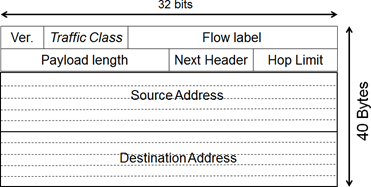
\includegraphics[scale = 0.7]{fig21.png}
	\caption{IPv6 Header}
	\label{fig:Graph21}
\end{figure}

Đầu tiên, ta có tiêu đề IPv6 cơ bản với kích thước cố định là 40 byte, tiếp theo là dữ liệu lớp trên và một số tiêu đề mở rộng tùy chọn, sẽ được mô tả sau. Như có thể thấy, có một số trường trong tiêu đề gói, cung cấp một số cải tiến so với tiêu đề IPv4: 
\begin{itemize}
	\item Số lượng trường đã giảm từ 12 xuống 8
	\item Tiêu đề IPv6 cơ bản có kích thước cố định là 40 byte và được căn chỉnh với 64 bit, cho phép chuyển tiếp gói dựa trên phần cứng nhanh hơn trên các bộ định tuyến
	\item Kích thước của địa chỉ tăng từ 32 lên 128 bit
\end{itemize}
Các trường quan trọng nhất là địa chỉ nguồn và địa chỉ đích. Như đã biết, mọi thiết bị IP đều có một địa chỉ IP duy nhất xác định nó trên Internet. Địa chỉ IP này được sử dụng bởi các bộ định tuyến để đưa ra quyết định chuyển tiếp của chúng. \\

Tiêu đề IPv6 có 128 bit cho mỗi địa chỉ IPv6, điều này cho phép 2128 địa chỉ (khoảng 3,4 × 1038, tức là 3,4 theo sau là 38 số 0), trong khi IPv4 sử dụng 32 bit để mã hóa mỗi trong số 232 địa chỉ (4.294.967.296) được phép. \\

Chúng ta đã thấy tiêu đề IPv6 cơ bản. Để giữ cho tiêu đề cơ bản đơn giản và có kích thước cố định, các tính năng bổ sung được thêm vào IPv6 bằng các tiêu đề mở rộng. \\

\begin{figure}[h]
	\centering
	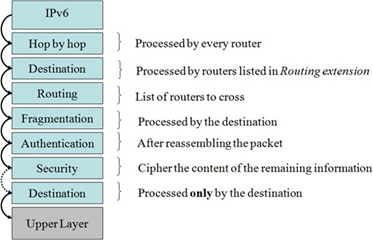
\includegraphics[scale = 0.7]{fig22.png}
	\caption{IPv6 Extension headers}
	\label{fig:Graph22}
\end{figure}

\textbf{Một số tiêu đề mở rộng đã được xác định, như có thể thấy trong hình trước, và chúng phải tuân theo thứ tự được hiển thị. Extension headers:}
\begin{itemize}
	\item Cung cấp tính linh hoạt, chẳng hạn, để kích hoạt bảo mật bằng cách mã hóa dữ liệu trong gói.
	\item Tối ưu hóa việc xử lý gói tin, bởi vì ngoại trừ tiêu đề hop by hop, các phần mở rộng chỉ được xử lý bởi các nút cuối, (nguồn và đích cuối cùng của gói tin), không phải bởi mọi bộ định tuyến trong đường dẫn.
	\item Chúng được đặt dưới dạng "chuỗi tiêu đề" bắt đầu luôn ở tiêu đề IPv6 cơ bản, sử dụng trường bên cạnh tiêu đề để trỏ đến tiêu đề mở rộng sau.
\end{itemize}
\textbf{Việc sử dụng 128 bit cho các địa chỉ mang lại một số lợi ích:}
\begin{itemize}
	\item Cung cấp nhiều địa chỉ hơn, để đáp ứng nhu cầu hiện tại và tương lai, với không gian rộng rãi để đổi mới
	\item Đơn giản hóa các cơ chế tự động cấu hình địa chỉ
	\item Quản lý / ủy quyền địa chỉ dễ dàng hơn
	\item Phòng cho nhiều mức phân cấp hơn và tổng hợp tuyến đường
	\item Khả năng thực hiện IPsec end-to-end
\end{itemize}
\textbf{Địa chỉ IPv6 được phân thành các loại sau:}
\begin{itemize}
	\item Unicast (one-to-one): được sử dụng để gửi một gói tin từ nguồn đến một đích duy nhất. 
	\item Multicast (một-nhiều): được sử dụng để gửi một gói từ nguồn đến một số đích. Điều này có thể thực hiện được nhờ định tuyến đa hướng cho phép các gói sao chép ở một số nơi.
	\item Anycast (một-đến-gần nhất): được sử dụng để gửi một gói từ nguồn đến đích gần nhất từ một tập hợp chúng.
	\item Dành riêng: Địa chỉ hoặc nhóm trong số đó cho các mục đích sử dụng đặc biệt.
\end{itemize}
Trước khi đi vào chi tiết hơn về địa chỉ IPv6 và các loại địa chỉ unicast, hãy xem chúng trông như thế nào và các quy tắc ký hiệu là gì
\begin{figure}[h]
	\centering
	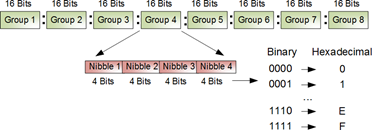
\includegraphics[scale = 0.7]{fig23.png}
	\caption{IPv6 address}
	\label{fig:Graph23}
\end{figure}. 

\textbf{Các quy tắc ký hiệu địa chỉ IPv6 là:}
\begin{itemize}
	\item 8 Nhóm 16 bit được phân tách bằng “:”
	\item Ký hiệu thập lục phân của mỗi nibble (4 bit)
	\item Không phân biệt chữ hoa chữ thường
	\item Tiền tố mạng (nhóm địa chỉ) được viết Tiền tố / Độ dài tiền tố, tức là độ dài tiền tố biểu thị số bit của địa chỉ chung cho nhóm
	\item Các số 0 tận cùng bên trái trong mỗi nhóm có thể bị loại bỏ
	\item Có thể thay thế một hoặc nhiều nhóm 0 bằng “::”. Điều này chỉ có thể được thực hiện một lần
\end{itemize}
\textbf{Sau đây là một số loại địa chỉ unicast khác:}
\begin{itemize}
	\item \textbf{Link-local:} Địa chỉ Link-local luôn có trong giao diện IPv6 được kết nối với mạng. Tất cả chúng đều bắt đầu bằng tiền tố FE80 :: / 10 và có thể được sử dụng để giao tiếp với các máy chủ khác trên cùng một mạng cục bộ, tức là tất cả các máy chủ được kết nối với cùng một switch. Chúng không thể được sử dụng để giao tiếp với các mạng khác, tức là để gửi hoặc nhận các gói thông qua bộ định tuyến.
	\item \textbf{ULA (Địa chỉ cục bộ duy nhất):} Tất cả các địa chỉ ULA đều bắt đầu bằng tiền tố FC00 :: / 7, trong thực tế có thể thấy FC00 :: / 8 hoặc FD00 :: / 8. Dành cho liên lạc cục bộ, thường là bên trong một trang web, chúng không được mong đợi sẽ được định tuyến trên Internet toàn cầu mà chỉ được sử dụng trong một môi trường hạn chế hơn.
	\item \textbf{Global Unicast:} Tương đương với các địa chỉ công cộng IPv4, chúng là duy nhất trên toàn bộ Internet và có thể được sử dụng để gửi một gói tin từ một trang web đến bất kỳ điểm đến nào trong Internet.
\end{itemize}

Như chúng ta đã thấy, IPv6 có một số tính năng hỗ trợ những thứ như định địa chỉ chung và tự động định cấu hình địa chỉ của máy chủ. Vì IPv6 cung cấp nhiều địa chỉ mà chúng ta có thể cần trong hàng trăm năm, nên chúng ta có thể đặt một địa chỉ IPv6 unicast toàn cầu cho hầu hết mọi thứ mà chúng ta có thể nghĩ đến. Điều này mang lại mô hình Internet ban đầu mà mọi thiết bị IP có thể giao tiếp với mọi thiết bị IP. Giao tiếp đầu cuối này cho phép giao tiếp hai chiều trên Internet và giữa bất kỳ thiết bị IP nào, điều này có thể dẫn đến các ứng dụng cộng tác và các cách mới để lưu trữ, gửi và truy cập thông tin.

Sự sẵn có của một lượng lớn địa chỉ đã cho phép một cơ chế mới được gọi là tự động định cấu hình địa chỉ không trạng thái (SLAAC) không tồn tại với IPv4. Dưới đây là tóm tắt ngắn gọn về các cách khác nhau để định cấu hình địa chỉ trên giao diện IPv6:
\begin{itemize}
	\item \textbf{Statically:} Bạn có thể quyết định địa chỉ nào bạn sẽ cấp cho thiết bị IP của mình và sau đó cấu hình thủ công địa chỉ đó vào thiết bị bằng bất kỳ loại giao diện nào: web, dòng lệnh, v.v. Thông thường, bạn cũng phải định cấu hình các thông số mạng khác như cổng vào để sử dụng để gửi các gói tin ra khỏi mạng của bạn.
	\item \textbf{DHCPv6} (Giao thức cấu hình máy chủ động cho IPv6): Một cổng của cơ chế tương tự đã có sẵn trong IPv4. Bạn cần định cấu hình một máy chủ chuyên dụng mà sau một cuộc thương lượng ngắn với thiết bị sẽ gán một địa chỉ IP cho nó. DHCPv6 cho phép các thiết bị IP được cấu hình tự động, đây là lý do tại sao nó được đặt tên là tự động cấu hình địa chỉ trạng thái, bởi vì máy chủ DHCPv6 duy trì trạng thái của các địa chỉ được chỉ định.
	\item \textbf{SLAAC:} Tự động định cấu hình địa chỉ không trạng thái [RFC4862] là một cơ chế mới được giới thiệu với IPv6 cho phép định cấu hình tự động tất cả các thông số mạng trên thiết bị IP bằng bộ định tuyến cung cấp kết nối với mạng.
\end{itemize}

Ưu điểm của SLAAC là nó đơn giản hóa cấu hình của các thiết bị " dumb", như cảm biến, máy ảnh hoặc bất kỳ thiết bị nào khác có công suất xử lý thấp. Bạn không cần sử dụng bất kỳ giao diện nào trong thiết bị IP để định cấu hình bất kỳ thứ gì, chỉ cần "cắm và kết nối mạng". Nó cũng đơn giản hóa cơ sở hạ tầng mạng cần thiết để xây dựng mạng IPv6 cơ bản, vì bạn không cần thiết bị / máy chủ bổ sung, bạn sử dụng cùng một bộ định tuyến mà bạn cần để gửi các gói bên ngoài mạng của mình để định cấu hình thiết bị IP. Chúng tôi sẽ không đi vào chi tiết, nhưng bạn chỉ cần biết rằng trong một mạng LAN (Mạng cục bộ), được kết nối với Internet bằng bộ định tuyến, bộ định tuyến này có nhiệm vụ gửi tất cả thông tin cấu hình cần thiết đến các máy chủ của nó bằng cách sử dụng một thông báo RA (Quảng cáo Bộ định tuyến). Bộ định tuyến sẽ gửi RA định kỳ, nhưng để đẩy nhanh quá trình, máy chủ có thể gửi một thông báo RS (Bộ định tuyến Solicitation) khi giao diện của nó được kết nối với mạng. Bộ định tuyến sẽ gửi RA ngay lập tức để phản hồi lại RS.

Hình sau cho thấy sự trao đổi gói giữa một máy chủ vừa kết nối với mạng cục bộ và một số đích IPv6 trên Internet:
\begin{figure}[h]
	\centering
	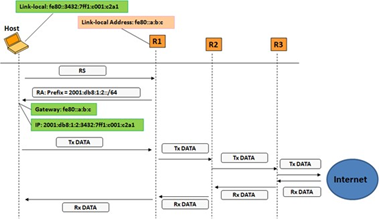
\includegraphics[scale = 0.7]{fig24.png}
	\caption{Packet exchange in IPv6}
	\label{fig:Graph24}
\end{figure}

\subsubsection{RPL - IPv6 Routing Protocol for Low-Power and Lossy Networks}
RPL là một giao thức định tuyến IPv6 cho các mạng có công suất thấp và mất gói được
thiết kế bởi IETF Routing Over Low và mạng Lossy (lossy network), được sử dụng làm giao
thức định tuyến De facto trong Contiki. RPL là một giao thức vector khoảng cách chủ động,
nó bắt đầu tìm kiếm các tuyến đường ngay khi mạng RPL được khởi tạo.
\begin{figure}[h]
	\centering
	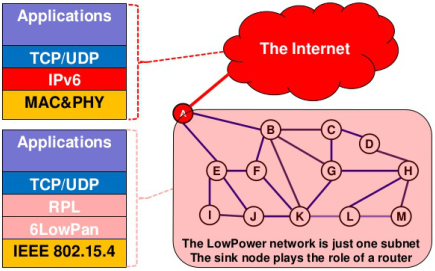
\includegraphics[scale = 0.7]{fig16.png}
	\caption{RPL trong protocol stack}
	\label{fig:Graph16}
\end{figure}

RPL hỗ trợ 3 kiểu traffic:
\begin{itemize}
\item Multipoint-to-point (MP2P).
\item Point-to-multipoint (P2MP).
\item Point-to-point (P2P). 
\end{itemize}

RPL xây dựng các đồ thị không tuần hoàn định hướng mục tiêu (DODAGs) có gốc
luôn hướng về một nguồn (DAG ROOT) được xác định bởi một định danh
DODAGID duy nhất. Các DODAGs được tối ưu hoá sử dụng một tiêu chí đo theo
hàm mục tiêu (OF) được xác định bởi một mã mục tiêu (OCP), dùng để chỉ ra các
ràng buộc động và các tiêu chí như số lượng hop, độ trễ, số lần truyền kỳ vọng, lựa
chọn mẫu, suy hao năng lượng… Một số hạng được gán cho mỗi nút có thể được sử
dụng để quyết định vị trí và khoảng cách tương đối của nó tới gốc trong DODAG.\\

\begin{figure}[h]
	\centering
	\subfigure[]{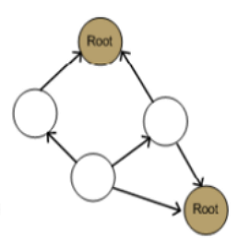
\includegraphics[scale = 0.7]{fig17.png}} 
	\subfigure[]{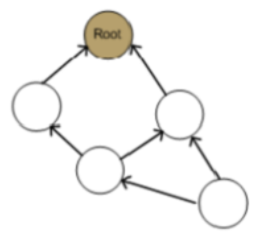
\includegraphics[scale = 0.7]{fig18.png}} 
	\caption{(a) DAG (b) DODAG }
	\label{fig:Graph17}
\end{figure}

\textbf{DAG: Đồ thị Acyclic có hướng Hình \ref{fig:Graph17} (a)}
\begin{itemize}
	\item DAG root: một nút trong DAG không có cạnh đi ra
	\item Tất cả các đường dẫn được kết thúc tại DAG root
\end{itemize}

\textbf{DODAG: DAG định hướng đích Hình \ref{fig:Graph17} (b)} 
\begin{itemize}
	\item Xác định một DAG tạo thành các đường dẫn đến một gốc lôgic duy nhất
\end{itemize} 

Một RPL Instance chứa một hoặc nhiều gốc DODAG. Một RPL Instance có thể cung cấp các tuyến đường đến các tiền tố đích nhất định, có thể truy cập được thông qua các gốc DODAG hoặc các đường dẫn thay thế trong DODAG. Các gốc này có thể hoạt động độc lập hoặc có thể phối hợp qua một mạng không nhất thiết bị ràng buộc như LLN. Một Phiên bản RPL có thể bao gồm:
\begin{itemize}
	\item Một DODAG với một gốc duy nhất: Một DODAG được tối ưu hóa để giảm thiểu độ trễ bắt nguồn từ một bộ điều khiển chiếu sáng tập trung duy nhất trong ứng dụng tự động hóa gia đình.
	\item Nhiều DODAG không phối hợp với các gốc độc lập (các DODAGID khác nhau): Nhiều điểm thu thập dữ liệu trong một ứng dụng thu thập dữ liệu đô thị không có kết nối phù hợp để phối hợp với nhau hoặc sử dụng sự hình thành nhiều DODAG như một phương tiện để phân vùng mạng một cách tự động.
	\item Một DODAG duy nhất có gốc ảo điều phối các LLN sinks (với cùng một DODAGID) trên mạng trục: Nhiều bộ định tuyến biên giới hoạt động với một liên kết chuyển tuyến đáng tin cậy, ví dụ: hỗ trợ ứng dụng 6LowPAN, có khả năng hoạt động như các giao diện tương đương về mặt logic với sink của cùng một DODAG.
\end{itemize}

\begin{figure}[h]
	\centering
	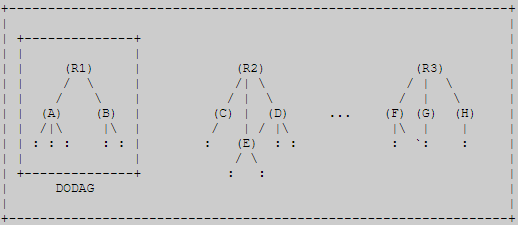
\includegraphics[scale = 0.7]{fig19.png}
	\caption{RPL Instance}
	\label{fig:Graph19}
\end{figure}

\textbf{Upward Routes và DODAG Construction:} Các điều khoản RPL hướng tới các gốc của DODAG, tạo thành một DODAG được tối ưu hóa theo một Chức năng Mục tiêu (OF). Các nút RPL xây dựng và duy trì các DODAG này thông qua các bản tin DODAG Information Object (DIO).
\begin{itemize}
	\item Hàm Mục tiêu (OF): Hàm Mục tiêu (OF) xác định cách các nút RPL chọn và tối ưu hóa các tuyến trong một RPL Instance. OF được xác định bằng Objective Code Point (OCP) trong tùy chọn Cấu hình DIO. OF xác định cách các nút dịch một hoặc nhiều các chỉ số và ràng buộc thành một giá trị được gọi là Rank, ước tính khoảng cách của nút từ gốc DODAG. OF cũng xác định cách các nút chọn parent. 
	\begin{figure}[h]
		\centering
		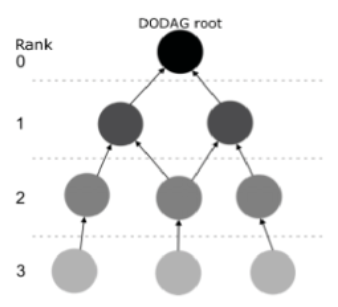
\includegraphics[scale = 0.7]{fig20.png}
		\caption{Rank}
		\label{fig:Graph20}
	\end{figure}
	\item RPL có hai cơ chế để sửa chữa topo của DODAG, một cơ chế để chống lặp và cho
	phép các nút gia nhập/gia nhập lại, cơ chế còn lại gọi là sửa chữa toàn cục. Sửa
	chữa toàn cục được khởi tạo tại DODAG ROOT bằng cách tăng số phiên bản
	DODAG để tạo một phiên bản DODAG mới.
\end{itemize}

\textbf{Downward Routes và Destination Advertisement:} RPL sử dụng các Destination Advertisement Object (DAO) để thiết lập các tuyến đi xuống. Thông báo DAO là một tính năng tùy chọn cho các ứng dụng yêu cầu lưu lượng P2MP hoặc P2P. RPL hỗ trợ hai chế độ lưu lượng truy cập xuống: lưu trữ (trạng thái hoàn toàn) hoặc không lưu trữ (định tuyến nguồn hoàn toàn). Bất kỳ Phiên bản RPL nhất định nào đều đang lưu trữ hoặc không lưu trữ. Trong cả hai trường hợp, các gói P2P di chuyển Lên tới Gốc DODAG rồi Xuống đến đích cuối cùng (trừ khi đích nằm trên lộ trình đi lên). Trong trường hợp không lưu trữ, gói tin sẽ di chuyển đến tận gốc DODAG trước khi di chuyển xuống. Trong trường hợp lưu trữ, gói tin có thể được hướng xuống đích bởi ancestor chung của nguồn và đích trước khi đến Gốc DODAG. \\

\textbf{Datapath Validation và Loop Detection:}
\begin{itemize}
	\item RPL mang thông tin định tuyến trong RPL Option được chứa trong IPv6 Hop-by-Hop Option. Thông tin định tuyến như vậy được sử dụng, ví dụ, để phát hiện vòng lặp trong DODAG và có thể được mở rộng trong các thông số kỹ thuật trong tương lai cho các tính năng bổ sung.
	\item Bản chất công suất thấp và tổn hao của LLN thúc đẩy việc sử dụng phát hiện vòng lặp theo yêu cầu của RPL bằng cách sử dụng các gói dữ liệu. Bởi vì lưu lượng dữ liệu có thể không thường xuyên, việc duy trì cấu trúc liên kết định tuyến liên tục được cập nhật với cấu trúc liên kết vật lý có thể lãng phí năng lượng. Các LLN điển hình thể hiện các biến thể trong kết nối vật lý tạm thời và vô hại đối với lưu lượng truy cập, nhưng điều đó sẽ tốn kém nếu theo dõi chặt chẽ từ mặt phẳng điều khiển. RPL không cần giải quyết các thay đổi nhất thời và không thường xuyên trong kết nối cho đến khi có dữ liệu để gửi. Khía cạnh này trong thiết kế của RPL dựa trên các giao thức LLN hiện có, được sử dụng nhiều cũng như bằng chứng triển khai và thử nghiệm rộng rãi về tính hiệu quả của nó.
	\item Mỗi gói dữ liệu bao gồm Rank của phía phát. Sự không nhất quán giữa quyết định định tuyến cho một gói (hướng lên hoặc hướng xuống) và mối quan hệ Rank giữa hai nút cho thấy một vòng lặp có thể xảy ra. Khi nhận được một gói tin như vậy, một nút sẽ tổ chức một hoạt động sửa chữa cục bộ.
	\item Ví dụ: nếu một nút nhận được một gói được gắn cờ là di chuyển theo hướng lên và nếu gói đó ghi rằng phía phát có Rank thấp hơn (thấp hơn) so với nút nhận, thì nút nhận có thể kết luận rằng gói đó không tiến triển theo hướng đi lên và DODAG không nhất quán.
\end{itemize}

\textbf{Creation of Upward routes – DIO messages:} Upward route cho phép một nút tham gia DODAG bằng cách khám phá những người hàng xóm là thành viên của DODAG mà bạn quan tâm và xác định một nhóm parent. Các chính sách chính xác để lựa chọn hàng xóm và parent phụ thuộc vào việc thực hiện và do OF điều khiển. Phần này chỉ định tập hợp các quy tắc mà các chính sách phải tuân theo để có khả năng tương tác.
\begin{itemize}
	\item Các nút được định cấu hình để trở thành DODAG roots
	\item Các DODAG roots quảng cáo sự hiện diện của chúng (liên kết với DODAG, chi phí định tuyến và các chỉ số liên quan) bằng cách gửi các bản tin DIO đa hướng cục bộ của liên kết tới tất cả các nút RPL.
	\item Các nút lắng nghe DIOs
	\begin{description}
		\item[-] Tham gia DODAG mới (do đó chọn DODAG parent)
		\item[-] Hoặc để duy trì một DODAG hiện có, theo OF được chỉ định
	\end{description}
	\item Các nút cập nhật các mục nhập bảng định tuyến cho các điểm đến được chỉ định bởi thông báo DIO
\end{itemize}

\textbf{Creation of Downward Routes - DAO Messages:} Phần này mô tả cách RPL phát hiện và duy trì các tuyến đi xuống. RPL xây dựng và duy trì các tuyến đi xuống với các Destination Advertisement Object (DAO) messages. Các tuyến đi xuống hỗ trợ các dòng P2MP, từ DODAG roots về phía leaves. Các tuyến đi xuống cũng hỗ trợ các luồng P2P: Các thông điệp P2P có thể chuyển đến DODAG root (hoặc common ancestor) thông qua một tuyến hướng lên, sau đó đi từ DODAG root đến đích thông qua một tuyến đi xuống. Đặc điểm kỹ thuật này mô tả hai chế độ mà một RPL Instance có thể lựa chọn để duy trì các tuyến đi xuống. Trong chế độ đầu tiên, được gọi là "storing", các nút lưu trữ các bảng định tuyến đi xuống cho DODAG con của chúng. Mỗi bước nhảy trên một đường đi xuống trong mạng lưu trữ sẽ kiểm tra bảng định tuyến của nó để quyết định bước tiếp theo. Trong chế độ thứ hai, được gọi là "non-storing", các nút không lưu trữ bảng định tuyến xuống. Các gói tin hướng xuống được định tuyến với các tuyến nguồn được điền bởi DODAG Root. RPL cho phép tối ưu hóa P2P một bước đơn giản cho cả mạng storing và non-storing. Một nút có thể gửi một gói P2P đến một người hàng xóm trực tiếp.
\begin{itemize}
	\item RPL sử dụng Destination Advertisement Object (DAO) messages để thiết lập các tuyến đi xuống
	\item DAO messages là một tính năng tùy chọn cho các ứng dụng yêu cầu lưu lượng P2MP hoặc P2P
	\item RPL supports two modes of downward traffic
	\begin{description}
		\item[-] Storing (fully statefull)
		\item[-] Non‐storing (fully source routed)
	\end{description}
\end{itemize}

\textbf{Non-storing Mode}
\begin{itemize}
	\item Ở chế độ non-storing, RPL định tuyến các thông báo xuống dưới bằng cách sử dụng định tuyến nguồn IP. Quy tắc sau áp dụng cho các nút ở chế độ non-storing.
	\begin{enumerate}
		\item Trường Địa chỉ gốc của Tùy chọn thông tin chuyển tuyến PHẢI chứa một hoặc nhiều địa chỉ. Tất cả các địa chỉ này PHẢI là địa chỉ DAO parent của người gửi
		\item Khi nhận được một DAO unicast, một nút PHẢI truyền tải thông tin về tuyến đường đi xuống được cập nhật lên trên. Node CÓ THỂ sử dụng bất kỳ parent nào trong tập parent. Thông tin về lộ trình đi xuống trong DAO message CÓ THỂ được tổng hợp với các DAO khác trước khi được truyền lên trên, điều này CÓ THỂ dẫn đến việc trì hoãn quá trình truyền như được mô tả bên dưới.
		\item Khi một nút loại bỏ một nút khỏi tập hợp DAO parent của nó, nó CÓ THỂ tạo một thông báo DAO mới với tùy chọn Thông tin chuyển tuyến được cập nhật.
	\end{enumerate}
	\item Trong chế độ non-storing, một nút sử dụng các DAO để báo cáo DAO parent của nó cho DODAG Root. DODAG Root có thể kết hợp một tuyến đường đi xuống đến một nút bằng cách sử dụng các DAO parent sets từ mỗi nút trong tuyến. Thông tin Trình tự đường dẫn có thể được sử dụng để phát hiện thông tin DAO cũ. Mục đích của việc tính toán lộ trình mỗi bước nhảy này là để giảm thiểu lưu lượng truy cập khi DAO parent thay đổi. Nếu các nút đã báo cáo các tuyến nguồn hoàn chỉnh, thì trên một DAO parent thay đổi toàn bộ DODAG con sẽ phải gửi các DAO mới đến DODAG Root. Do đó, ở chế độ non-storing, một nút có thể gửi một DAO duy nhất, mặc dù nó có thể chọn gửi nhiều hơn một thông báo DAO cho mỗi parent của nhiều DAO.
	\item Các nút đóng gói DAO bằng cách gửi một tin nhắn DAO với nhiều Tùy chọn mục tiêu RPL. Mỗi Lựa chọn Mục tiêu RPL có các tùy chọn Thông tin Chuyển tuyến.
\end{itemize}
\textbf{Storing Mode}
\begin{itemize}
	\item Trong chế độ storing, RPL định tuyến các thông báo xuống theo địa chỉ đích IPv6. Quy tắc sau áp dụng cho các nút đang ở chế độ storing:
	\begin{enumerate}
		\item Trường Địa chỉ gốc của tùy chọn Thông tin truyền PHẢI để trống.
		\item Khi nhận một DAO unicast, một nút PHẢI tính toán xem DAO có thay đổi tập hợp các tiền tố mà chính nút đó quảng cáo hay không. Tính toán này NÊN bao gồm việc tham khảo thông tin Trình tự đường dẫn trong tùy chọn Thông tin chuyển tuyến được liên kết với DAO, để xác định xem thông báo DAO có chứa thông tin mới hơn thay thế thông tin đã được lưu trữ tại nút hay không. Nếu vậy, nút PHẢI tạo một thông báo DAO mới và truyền nó. Một sự thay đổi như vậy bao gồm cả việc nhận được DAO Không có Đường dẫn.
		\item Khi một nút tạo ra một DAO mới, nó NÊN kết hợp nó với từng DAO parent của nó. Nó KHÔNG ĐƯỢC hủy phát thông điệp DAO tới các nút không phải là parent của DAO.
		\item Khi một nút loại bỏ một nút khỏi tập hợp DAO parent của nó, nó NÊN gửi một thông báo DAO Không có đường dẫn đến nguồn gốc DAO đã bị loại bỏ đó để làm mất hiệu lực của tuyến đường hiện có.
		\item Nếu thư đến một địa chỉ được quảng cáo đi xuống bị lỗi chuyển tiếp, phát hiện không thể truy cập hàng xóm (NUD) hoặc lỗi tương tự, một nút CÓ THỂ đánh dấu địa chỉ là không thể truy cập và tạo DAO Không Đường dẫn thích hợp.
	\end{enumerate}
	\item Các DAO quảng cáo địa chỉ đích và tiền tố nào mà một nút có các tuyến đến. Không giống như ở chế độ non-storing, các DAO này không tự giao tiếp thông tin về các tuyến đường: thông tin đó được lưu trữ trong mạng và được ngầm định từ địa chỉ nguồn IPv6. Khi một nút lưu trữ tạo ra một DAO, nó sử dụng trạng thái được lưu trữ của các DAO mà nó đã nhận được để tạo ra một tập hợp các tùy chọn Mục tiêu RPL và các tùy chọn Thông tin truyền liên quan của chúng.
	\item Bởi vì thông tin này được lưu trữ trong các bảng định tuyến của mỗi nút, ở chế độ storing, các DAO được truyền trực tiếp đến các parent của DAO, những người này lưu trữ thông tin.
\end{itemize}
Mặc định Contiki sử dụng storing mode cho các tuyến đường RPL xuống. Về mặt
cơ bản, tất cả các nút lưu trữ trong một bảng định tuyến địa chỉ các nút con của
chúng.
\subsection{Adaptation Layer}
Network layer chứa hai lớp con, IPv6 layer ở trên và Adaptation layer ở dưới. Adaptation Layer cung cấp tính năng nén và phân mảnh tiêu đề của IPv6 và UDP để vận chuyển các gói IPv6 qua IEEE 802.15.4. \\

\textbf{Tại sao là 6LoWPAN ?} \\

Có rất nhiều ứng dụng có lợi được nhúng vào Internet không dây. Ngày nay các ứng dụng
này được triển khai bằng cách sử dụng nhiều công nghệ độc quyền, rất khó để tích hợp vào
các mạng lớn hơn và với các dịch vụ dựa trên Internet. Lợi ích của việc sử dụng các giao thức
Internet trong các ứng dụng này, và do đó tích hợp chúng với Internet of Things bao gồm
[RFC49109]:
\begin{itemize}
	\item Các thiết bị dựa trên IP có thể kết nối dễ dàng với các mạng IP khác mà không cần gateway
	dịch hoặc proxy
	\item Các mạng IP cho phép sử dụng cơ sở hạ tầng mạng hiện có
	\item Các công nghệ dựa trên IP đã tồn tại hàng thập kỷ, rất nổi tiếng, và đã được chứng minh là
	hoạt động hiệu quả và quy mô lớn. API - IPSocket (giao diện lập trình ứng dụng) là một trong
	những API được biết đến nhiều nhất và được sử dụng rộng rãi trên thế giới
	\item Công nghệ IP được chỉ định một cách mở và miễn phí, với các quy trình tiêu chuẩn và nhiều
	tài liệu sẵn có cho bất cứ ai. Kết quả là công nghệ IP khuyến khích đổi mới và được hiểu rõ
	với phần đông người dùng
	\item Công cụ quản lý, vận hành và chẩn đoán mạng IP đã và đang tồn tại, tuy vẫn phải tối ưu
	để hỗ trợ nhiều giao thức cho việc sử dụng trực tiếp với các node 6LoWPAN. Cho đến nay,
	các thiết bị và mạng nhúng trở nên cực kì mạnh mẽ đã có thể tham gia trực tiếp với Internet.
\end{itemize}

	Truyền thông trực tiếp với các mạng IP truyền thống đòi hỏi nhiều giao thức Internet, thường
đòi hỏi một hệ điều hành để đối phó với sự phức tạp và khả năng bảo trì. Các giao thức Internet
truyền thống đòi hỏi các thiết bị nhúng vì những lý do sau: 
\begin{itemize}
	\item Bảo mật: IPv6 bao gồm hỗ trợ tùy chọn cho việc xác thực và mã hóa IP Security (IPsec) và
	các dịch vụ web thường sử dụng các socket an toàn hoặc các cơ chế bảo mật tầng vận chuyển.
	Những kỹ thuật này có thể quá phức tạp, đặc biệt đối với các thiết bị nhúng đơn giản
	\item Các dịch vụ Web: Các dịch vụ Internet ngày nay dựa vào các dịch vụ web, chủ yếu sử dụng
	giao thức điều khiển truyền dẫn (TCP), HTTP, SOAP và XML với các mẫu giao dịch phức
	tạp.
	\item Quần lý: Quản lý với giao thức quản lý mạng đơn giản (SNMP) và các dịch vụ web thường
	không hiệu quả và phức tạp.
	\item Kích thước khung: Các giao thức Internet hiện tại yêu cầu các liên kết với độ dài khung đầy
	đủ (tối thiểu 1280 byte cho IPv6) và các giao thức ứng dụng nặng đòi hỏi băng thông đáng kể.
\end{itemize}

Các yêu cầu này đã giới hạn Internet of Things cho các thiết bị với một bộ xử lý mạnh mẽ,
một hệ điều hành với một ngăn xếp TCP/IP đầy đủ, và một liên kết truyền thông có khả năng
IP. Các thiết bị Internet tiêu biểu hiện nay bao gồm các thiết bị công nghiệp với giao diện
Ethernet, cổng M2M với modem di động và điện thoại thông minh tiên tiến. Phần lớn các ứng
dụng nhúng liên quan đến thiết bị hạn chế sử dụng mạng không dây. Các thiết bị và mạng
nhúng không dây đặc biệt gặp nhiều thách thức đối với các giao thức Internet:
\begin{itemize}
	\item Chu kỳ công suất và chu kỳ hoạt động: Các thiết bị không dây chạy bằng pin cần phải giữ
	chu kỳ hoạt động thấp (phần trăm thời gian hoạt động). Giả định cơ bản của IP là một thiết
	bị luôn được kết nối.
	\item Multicast: Các công nghệ vô tuyến không dây nhúng, chẳng hạn như IEEE 802.15.4, thường
	không hỗ trợ multicast, và flooding trong một mạng như vậy là lãng phí điện năng và băng
	thông. Multicast là rất quan trọng đối với hoạt động của nhiều tính năng IPv6.
	\item Mesh topologies: Các ứng dụng của công nghệ radio không dây nhúng thường được lợi từ
	mạng lưới multihop lưới để đạt được yêu cầu và hiệu quả chi phí. Các giải pháp định tuyến IP
	hiện tại có thể không dễ áp dụng cho các mạng như vậy.
	\item Băng thông và kích thước khung: Công nghệ vô tuyến điện không dây công suất thấp thường
	có băng thông giới hạn (khoảng 20-250 kbit/giây) và kích thước khung (khoảng 40 đến 200
	byte). Trong các cấu trúc liên kết lưới, băng thông giảm thêm khi kênh được chia sẻ và nhanh
	chóng bị giảm bởi chuyển tiếp đa giao diện. Chuẩn IBEE 802.15.4 có kích thước khung 127
	byte, với kích thước tải trọng lớp 2 thấp tới 72 byte. Kích thước khung tối thiểu cho IPv6 tiêu
	chuẩn là 1280 byte [REC2460], do đó yêu cầu phân mảnh.
	\item Độ tin cậy: Các giao thức Internet tiêu chuẩn không được tối ưu hóa cho các mạng không dây
	công suất thấp. Ví dụ, TCP không có khả năng phân biệt giữa các gói bị giảm do tắc nghẽn
	hoặc các gói bị mất trên các liên kết không dây. Hơn nữa sự không đáng tin cậy xảy ra trong
	mạng không dây nhúng vì sự thất bại của nút, sự cạn kiệt năng lượng và các chu kỳ nhiệm vụ
	ngủ.
\end{itemize}

Nhóm làm việc ITEF 6LoWPAN đã được tạo ra để giải quyết những vấn đề này
và đặc biệt cho phép IPv6 được sử dụng với các thiết bị không dây và mạng nhúng. Các tính
năng của thiết kế IPv6 như cấu trúc tiêu đề đơn giản, và mô hình định vị theo cấp bậc, làm
cho nó trở nên lý tưởng để sử dụng trong các mạng nhúng không dây với 6LoWPAN. Ngoài ra,
bằng cách tạo ra một nhóm tiêu chuẩn dành cho các mạng này, yêu cầu tối thiểu cho việc triển
khai một ngăn xếp IPv6 nhẹ với 6LoWPAN có thể được liên kết với các thiết bị tối thiểu. Cuối
cùng bằng cách thiết kế một phiên bản của Neighbor Discovery (ND) đặc biệt cho 6LoWPAN,
đặc tính riêng của mạng lưới điện không dây công suất thấp có thể được tính đến. Kết quả
của 6LoWPAN là sự mở rộng hiệu quả của IPv6 vào miền không dây nhúng, do đó cho phép
kết nối mạng IP end-to-end và các tính năng cho một loạt các ứng dụng nhúng. Tham khảo
[RFC4919] để biết các giả định chi tiết, tuyên bố vấn đề và mục tiêu của tiêu chuẩn 6LoWPAN
ban đầu. Mặc dù 6LoWPAN đã được nhắm mục tiêu theo chuẩn IEEE 802.15.4 và giả định
chuyển tiếp lớp 2-RFC [RFC4944], nó đã được tổng quát hoá cho tất cả các công nghệ liên kết
tương tự, với sự hỗ trợ thêm cho định tuyến IP trong [ID-6LoWPAN-hc, ID-6LoWPAN-nd]. \\
\newpage
\textbf{6LoWPAN - IPv6 over Low-power Wireless Personal Area Networks}
\begin{figure}[h]
	\centering
	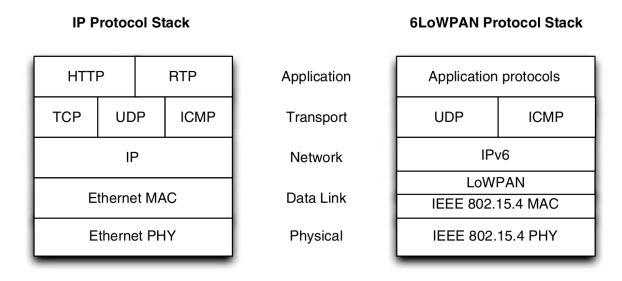
\includegraphics[scale = 0.7]{fig25.png}
	\caption{IP and 6LoWPAN protocol stacks}
	\label{fig:Graph25}
\end{figure}

Chúng ta đã thấy rằng có một lớp thấp hơn (lớp PHY và lớp LINK trên mô hình ngăn xếp
TCP/IP) cung cấp kết nối tới các thiết bị trong cái được gọi là LoWAN. Đồng thời sử dụng
IPv6 trên lớp này sẽ mang lại nhiều lợi ích. Lý do chính để phát triển các tiêu chuẩn IETF
được đề cập trong phần giới thiệu là giữa IP (lớp mạng) và tầng dưới có một số vấn đề quan
trọng cần giải quyết bằng một lớp Adaptation, chính là 6LoWPAN với các mục tiêu được trình
bày ngay sau đây. \\

Lớp Fragmentation và Reassembly: Đặc tả IPv6 [RFC2460] xác định rằng MTU tối thiểu mà
một lớp liên kết nên cung cấp cho lớp IPv6 là 1280 byte. Giao thức các đơn vị dữ liệu có thể chứa 81 byte theo chuẩn IEEE 802.15.4. Để giải quyết sự khác biệt trong lớp phân mảnh và
tái lắp ráp phải được cung cấp ở lớp dưới IP. \\
\begin{figure}[h]
	\centering
	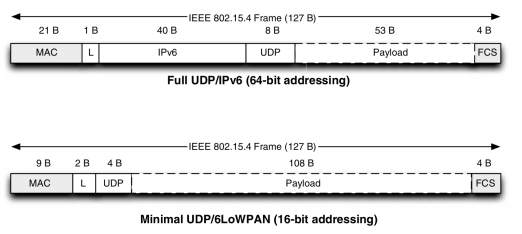
\includegraphics[scale = 0.7]{fig26.png}
	\caption{6LoWPAN nén header}
	\label{fig:Graph26}
\end{figure}

Header Compression - Nén header: Trong trường hợp xấu nhất, kích thước tối đa có sẵn
để truyền các gói tin IP trên một khung IEEE 802.15.4 là 81 octet, và header IPv6 là 40
octet chiều dài (không có header mở rộng tùy chọn), vậy chỉ để lại 41 octet cho các giao thức
upperlayer, như UDP và TCP. UDP sử dụng 8 octets trong header và TCP sử dụng 20 octet.
Vậy chỉ còn lại 33 octet dữ liệu qua UDP và 21 octet cho dữ liệu qua TCP. Thêm vào đó, như
đã đề cập ở trên, cũng cần phải có một lớp Fragmentation và Reassermbly, điều này sẽ sử dụng
nhiều octet để lại rất ít octet cho dữ liệu. Do đó, nếu người ta sử dụng các giao thức như vậy
thì nó sẽ dẫn đến phân mảnh và tái lắp ráp quá mức, ngay cả khi các gói dữ liệu chỉ dài 10
giây. Diều này cho thấy sự cần thiết phải nén header. \\

Address Autoconfiguration - Tự cấu hình địa chỉ : xác định các phương pháp để tạo địa
chỉ IPv6 tự động cấu hình (đối lập với stateful) cho phù hợp 6LoWPANs, vì nó làm
giảm câu hình overhead trên máy chủ. Cần có một phương pháp để tạo ra IPv6 IID (Interface
Identifer) từ EUI-64 được gắn cho thiết bị IEEE 802.15.4. \\

Mesh Routing Protocol - Giao thức Routing mạng Mesh: Một giao thức định tuyến để hỗ
trợ mạng lưới multi-hop là cần thiết. Cần cẩn thận khi sử dụng các giao thức định tuyến hiện
tại (hoặc thiết kế các giao thức mới) để các gói tin định tuyến phù hợp trong một khung IEEE
802.15.4. Các cơ chế được xác định bởi IETF WLAN 6LoWPAN dựa trên một số yêu cầu đối
với lớp IEEE 802.15.4. \\

IEEE 802.15.4 định nghĩa bốn loại khung: khung beacon, khung MAC command, khung xác
nhận (acknowledgement) và khung dữ liệu. Các gói IPv6 phải được mang trên các khung dữ
liệu. Khung dữ liệu có thể yêu cầu rằng nó được xác nhận và cho phép các khung trong đó địa
chỉ nguồn hoặc đích (hoặc cá hai) được xóa bỏ. Cả hai địa chỉ nguồn và đích đều phải được
bao gồm trong header khung IEEE 802.15.4. Các trường PAN ID nguồn hoặc đích cũng có thể
được gói kèm trong gói tin. Tiêu chuẩn 6LoWPAN giả định rằng một PAN sắp xếp đến một
liên kết IPv6 cụ thể. Cả hai địa chỉ mở rộng 64-bit và địa chỉ ngắn 16-bit đều được hỗ trợ.
Multicast không được hỗ trợ trong IEEE 802.15.4. Do đó, các gói multicast cấp độ IPv6 phải
được thực hiện như các khung broadcast ở lớp link trong mạng IEEE 802.15.4. \\

6LoWPAN được chỉ định để mang các gói tin IPv6 qua các liên kết bị ràng buộc, có tính đến
băng thông, bộ nhớ, hoặc nguồn năng lượng hạn chế trong các ứng dụng như mạng cảm biến
không dây. Đối với mỗi mục tiêu và yêu cầu này, có các giải pháp được cung cấp bởi 6LoWPAN:
\begin{itemize}
	\item Một header địa chỉ mạng Mesh để hỗ trợ chuyển tiếp sub-IP
	\item Một header phân mảnh để hỗ trợ IPv6 tối thiểu yêu cầu MTU
	\item Một Header broadcast được sử dụng khi gói tin multicast IPv6 qua mạng IEEE 802.15.4
	\item Nén Stateless Header cho phép các gói tin IPv6 giảm độ lớn header IPv6 và UDP xuống
	một vài byte. Header này được sử dụng cho việc đóng gói LoWPAN và có thể được sử dụng
	đồng thời tạo thành ngăn xếp header. Mỗi header trong ngăn xếp chứa là một loại header
	theo sau bởi không hoặc nhiều trường header. Khi có nhiều hơn một header LoWPAN được sử
	dụng trong cùng một gói tin, chúng phải xuất hiện theo thứ tự sau: Mesh Addressing Header,
	Broadcast Header, và Fragmentation Header
\end{itemize}
\newpage
\begin{figure}[h]
	\centering
	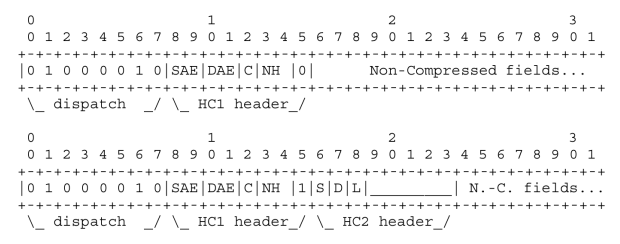
\includegraphics[scale = 0.7]{fig27.png}
	\caption{Nén header trong 6LoWPAN}
	\label{fig:Graph27}
\end{figure}

\textbf{IPv6 Interface Identifer (IID):} Như đã nói, một thiết bị IEEE 802.15.4 có thể có hai loại
địa chỉ. Đối với mỗi một loại có một cách khác nhau để tạo ra IPv6 IID. Địa chỉ IEEE EUI-61:
"Tất cả các thiết bị đều có loại địa chỉ này. Irong trường hợp này, Interface Identifiier được hình
thành từ EUI-64, bổ sung cho "Universal/Local" (U / L) bit, là bit gần bit thấp nhất của octet
đầu tiên của EUI-641. Việc bổ sung bit này nói chung sẽ thay đổi giá trị 0 thành 1. Địa chỉ ngắn
16 bit: Có thể nhưng không phải lúc nào cũng được sử dụng. IPv6 IID được hình thành bằng
cách sử dụng PAN (hoặc zero trong trường hợp không biết PAN) và địa chỉ ngắn 16 bit. \\

\textbf{Header Compression:} Hai định dạng mã hóa được định nghĩa cho nén các gói tin IPv6:
LoWPAN-IPHC và LoWPAN-NHC, định dạng mã hóa cho header tiếp theo tùy ý. Để cho phép
nén hiệu quả, LoWPAN-IPHC dựa vào thông tin liên quan đến toàn bộ 6LoWPAN.

\begin{figure}[h]
	\centering
	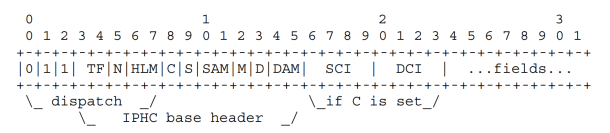
\includegraphics[scale = 0.7]{fig28.png}
	\caption{Nén Header LoWPAN-IPHC}
	\label{fig:Graph28}
\end{figure}

Trong đó:
\begin{itemize}
	\item TF: Traffic Class, Plow Label
	\item NH: Next Header
	\item HLIM: Hop Lìmit
	\item CID: Context Identifer Extension
	\item SAC: Source Address Compression
	\item SAM: Source Address Mode
	\item M: Multicast Compression
\end{itemize}
\newpage
Đối với việc mở rộng header, ta dùng LOWPAN-NHC được định dạng như sau:

\begin{figure}[h]
	\centering
	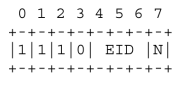
\includegraphics[scale = 0.7]{fig29.png}
	\caption{Nén Header LOWPAN-NHG}
	\label{fig:Graph29}
\end{figure}

Trong đó:
\begin{itemize}
	\item EID: IPv6 Extension Header ID
	\item 0; IPv6 Hop-by-Hop Options Header
	\item l; IPv6 Routing Header
	\item 2: IPv6 Fragment Header
	\item 3: IPv6 Destination Options Header
	\item 4: IPv6 Mobility Header
	\item 5: Reserved
	\item 6: Reserved
	\item 7: IPv6 Header
	\item NH: Next Header
	\begin{description}
		\item[-] 0: Toàn bộ 8 bit cho Next Header được gói trong hàng
		\item[-] 1: Trường Next Header được lược đi và mã hóa bằng cách sử dụng LOWPAN- NHC. Đối
		với hầu hết các phần, phần mở rộng header IPv6 được thực hiện không làm thay đổi các byte
		ngay sau bộ đếm LOWPAN-NHC
	\end{description}
\end{itemize}

\textbf{Tối ưu hóa NDP} \\

IEEE 802.15.4 và các công nghệ liên kết tương tự khác giới hạn hoặc không sử
dụng tín hiệu multicast để bảo tồn năng lượng. Thêm nữa, mạng không dây có thể
không tuân thủ chặt chẽ khái niệm IP subnets và IP links. Giao thức phát hiện mạng
bên cạnh IPv6 (NDP) không được thiết kết cho các liên kết không dây phi chuyển
tiếp, do khái niệm liên kết IPv6 truyền thống và việc sử dụng nhiều multicast làm
giảm hiệu quả và đôi khi bất khả thi trong một mạng không dây và suy hao. \\

Vì lý do này, một vài tối ưu đơn giản được định nghĩa cho IPv6 NDP. Cơ chế đánh
địa chỉ và xác định định chỉ trùng lặp của nó là: 
\begin{itemize}
	\item Tương tác khởi tạo host cho phép host ở chế độ sleeping
	\item Loại bỏ giải pháp multicast cho các host
	\item Tính năng đăng ký địa chỉ của một host sử dụng lựa chọn mới với các bản tin NS
	(Neighbor Solicitation) và NA (Neighbor Advertisement)
	\item Lựa chọn ND mới phân tán ngữ cảnh nén tiêu đề 6LoWPAN cho các host
	\item Phân tán multihop của tiền tố và ngữ cảnh nén tiêu đề 6LoWPAN
	\item Phát hiện trùng lặp địa chỉ multihop (DAD), sử dụng hai loại bản tin ICMPv6
	mới
\end{itemize}
\subsection{MAC Layer}
Giao thức điều khiển truy cập phương tiện MAC mô tả cách thức truy cập phương
tiện thông qua một mạng, bằng cách chỉ ra khi nào một nút nhất định được phép
truyền các gói tin. Các giao thức có thể phân loại thành giao thức dựa trên cạnh
tranh và giao thức đặt trước. \\

Giao thức đầu tiên dựa trên cảm nhận sóng mang bằng cách phát hiện các hoạt động
trên phương tiện và dẫn đến xung đột cũng như hiệu quả thấp hơn khi tải nặng, tuy
nhiên lại dễ dàng cài đặt. Nhóm giao thức thứ hai lại hiệu quả về mặt thông lượng
và năng lượng, nhưng yêu cầu đồng bộ chính xác và ít thích nghi hơn với lưu lượng
truy cập động. \\

Cài đặt điều khiển truy cập phương tiện trong Contiki gồm 3 loại: Framer, Chu trình
nhiệm vụ vô tuyến (RDC) và điều khiển truy nhập phương tiện (MAC). Tầng mạng
có thể được truy cập thông qua các biến toàn cục: NETSTACK\_FRAMER,
NETSTACK\_RDC và NETSTACK\_MAC được định nghĩa tại thời gian dịch. Các
biến được đặt tại core/net/netstack.h.
\begin{figure}[h]
	\centering
	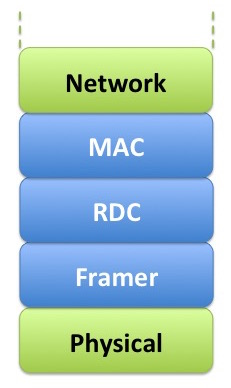
\includegraphics[scale = 0.7]{fig30.png}
	\caption{Các tầng giao thức Contiki Mac}
	\label{fig:Graph30}
\end{figure}
\subsubsection{Trình điều khiển MAC}
Contiki cung cấp hai trình điều khiển MAC: CSMA và nullMAC. \\

\textbf{Đa truy cập dựa trên cảm nhận sóng mang (CSMA):} nhận các gói tin đến từ tầng
RDC và sử dụng tầng RDC để truyến gói tin. Nếu tầng RDC hoặc tầng vô tuyến
phát hiện đường truyền đang bận, tầng MAC có thể truyền lại gói tin lại một thời
điểm sau đó. Giao thức CSMA giữ một danh sách và gói tin đã gửi tới các mạng
bên cạnh và tính toán các thông kê như số lần truyền lại, xung đột, trì hoãn,… Kiểm
tra truy cập phương tiện được thực hiện bởi trình điều khiển RDC. \\

\textbf{NullMAC:} là giao thức đơn giản. Ỏ lớp này không lắng nghe kênh truyền nên giảm thời gian
gửi nhưng tình trạng xung đột gói tin tăng lên rất cao, tỉ lệ mất gói lớn. 
\subsubsection{Trình điều khiển RDC}
Tầng chu trình nhiệm vụ vô tuyến RDC quản lý khoảng thời gian nghỉ của các nút.
Tầng này quyết định khi nào các gói tin sẽ được truyền và đảm bảo rằng các nút
được đánh thức khi các gói tin được nhận. \\

Cài đặt giao thức RDC của Contiki sẵn có trong core/net/mac. Các trình điều khiển
RDC sau được cài đặt: contikimac, xmac, lpp, nullrdc và sicslowmac. Hầu hết các
trường hợp sử dụng là ContikiMac. NullRDC là tầng truyền thông không bao giờ tắt
tín hiệu vô tuyến. \\

Các trình điều khiển RDC luôn cố gắng tắt tín hiệu vô tuyến nhiều nhất có thể, định
kỳ kiểm tra phương tiện không dây cho các hoạt động vô tuyến. Khi có hoạt động
được phát hiện, tín hiệu vô tuyến được bật để kiểm tra xem nếu nó phải nhận gói
tin, hay nó có thể quay lại trạng thái nghỉ. \\

Tần suất kiểm tra kênh được tính theo Hz, chỉ ra số lần kênh được kiểm tra trên 1
giây, và tần suất kiểm tra mặc định là 8 Hz. Các tần suất kiểm tra kênh được tính
theo số mũ của 2, thường là 2, 4, 8 và 16 Hz. 
\subsubsection{Trình điều khiển Framer}
Trình điều khiển Framer thực chất là một tập các hàm đối với khung dữ liệu được
truyền, và để phân tích dữ liệu nhận được. Cài dặt Framer được đặt tại core/net/mac,
với hai cài đặt cần lưu ý là framer-802154 và framer-nullmac. \\

Khi sử dụng IPv6, cần lựa chọn framer-802154. Trong các trường hợp ngược lại,
contikimac\_framer được sử dụng. \\

Framer-802154 được cài dặt rong core/net/mac/framer-802154.c. Trình điều khiển
khung dữ liệu tuân theo chuẩn IEEE 802.15.4. Framer chèn và tách dữ liệu từ cấu
trúc packetbuf.
\subsection{802.15.4 Physical Layer}
Lớp vật lý (Phygical Layer) là lớp thấp nhất trong mô hình tham chiếu OSI được sử dụng
trên toàn thế giới. Lớp vật lý là lớp cuối cùng cung cấp dịch vị truyền dữ liệu, cũng như giao
diện cho thực thể quản lý lớp vật lý, cho phép truy cập vào mọi chức năng quản lý mọi lớp và
duy trì cơ sở dữ liệu thông tỉn về các mạng cá nhân có liên quan (WPAN). Do đó, nó quản lý
bộ thu phát RF vật lý và thực hiện chức năng lựa chọn kênh và các chức năng quản lý năng
lượng và tín hiệu. Nó chuyển đổi các bit dữ liệu thành tín hiệu có thể truyền và nhận qua không
gian tự do. Nó hoạt động trên một trong ba dải tần số:
\begin{itemize}
	\item 868.0-868.6 MHz: Châu Âu, cho phép một kênh truyền thông (2003,2006,2011)
	\item 902-928 MHz: Bắc Mỹ, lên đến mười kênh (2003), kéo dài đến ba mươi (2006)
	\item 2400-2483.5 MHz: sử dụng trên toàn thế giới, lên đến mười sáu kênh (2003, 2006)
\end{itemize}
\begin{figure}[h]
	\centering
	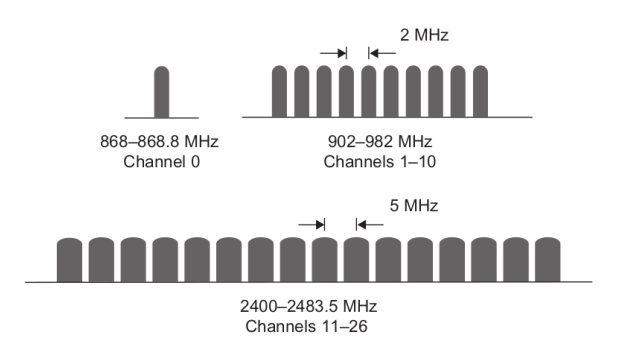
\includegraphics[scale = 0.7]{fig31.png}
	\caption{Các lựa chọn băng tần cho IEEE 802.15.4}
	\label{fig:Graph31}
\end{figure}

Ở Contiki, lớp PHY hỗ trợ hai băng tần: 1 ở tần số dưới 1 GHz và 1 ở 2.4GHz với 26
channel. Do băng tần 2.4 GHz cũng được sử dụng bởi các công nghệ khác như Wifi hay
Bluetooth, phổ tần này có thể bị chia sẻ và trùng lặp có thể xảy ra. Hình vẽ dưới đây
thể hiện việc phân bổ kênh cho 2.4 GHz IEEE 802.15.4, và các kênh được khuyến
nghị để tránh nhiễu với các thiết bị khác nằm cùng chỗ. Với sự tăng trưởng nhanh
của Bluetooth năng lượng thấp và sự phổ biến của Wifi trong hệ thống thường nhật,
việc lựa chọn kênh hoạt động hợp lý là thiết yếu trong bất kỳ triển khai IEEE
802.15.4 nào.
\begin{figure}[h]
	\centering
	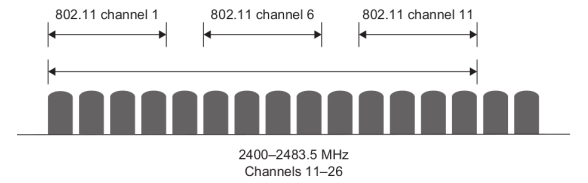
\includegraphics[scale = 0.7]{fig32.png}
	\caption{Phân bố kênh truyền giữa 6LoWPAN và Wifi}
	\label{fig:Graph32}
\end{figure}

\section{Bảo mật}
\subsection{Bảo mật trong mạng 6LoWPAN}
Internet trong tương lai là mạng IPv6 kết nối các máy tính truyền thống và một số lượng lớn các đối tượng thông minh. Các đối tượng thông minh, thường được gọi là vật, thường có các máy tính nhúng nhỏ với khả năng giao tiếp, cảm biến và hoạt động. Kết nối Internet of Things (IoT) sẽ là nền tảng cho nhiều dịch vụ và sẽ cho phép giao tiếp giữa máy tính truyền thống và các đối tượng thông minh trên quy mô toàn cầu. Do đó, điều quan trọng là phải giải quyết các yêu cầu bảo mật truyền thống, đó là xác thực, tính toàn vẹn, tính không từ chối và tính bảo mật trong bối cảnh của IoT. \\

Các đối tượng thông minh thường được kết nối với nhau bằng mạng IEEE 802.15.4 không dây. Border-router được sử dụng để kết nối mạng 802.15.4 với Internet để cho phép giao tiếp IPv6 giữa các đối tượng thông minh và máy chủ Internet. Tuy nhiên, các gói IPv6 di chuyển trên mạng 802.15.4 sử dụng định dạng tiêu đề nén như được xác định bởi IPv6 Over Low-power Wireless Personal Area Networks (6LoWPAN) để tiết kiệm tài nguyên băng thông khan hiếm. Border-router phải nén / giải nén tiêu đề gói IP khi chuyển tiếp gói để đảm bảo khả năng tương thích với Internet hiện có. \\

Hiện tại, 6LoWPAN dựa trên bảo mật 802.15.4 để bảo vệ giao tiếp giữa các nút lân cận. Tiêu chuẩn này hỗ trợ kiểm soát truy cập, tính toàn vẹn của bản tin, tính bảo mật và bảo vệ phát lại. Tính toàn vẹn của bản tin đạt được bằng cách bao gồm message authentication code (MAC) trong các gói. Nếu người nhận không thể xác minh MAC, gói tin sẽ bị loại bỏ. Tính bảo mật được cung cấp bằng cách áp dụng mật mã đối xứng cho các gói gửi đi. Thông qua việc bao gồm một bộ đếm tăng đơn điệu trong các messages, các nút có thể loại bỏ các gói được gửi lại bởi các nút độc hại, đạt được khả năng bảo vệ phát lại. \\

Hình \ref{fig:Graph52} cho thấy cấu trúc của một gói 802.15.4 với các tiêu đề bảo mật tùy chọn. Chi phí gói tin với Link Layer Security (LLSEC) thay đổi từ 4 đến 21 byte tùy thuộc vào sơ đồ được sử dụng.
\begin{figure}[h]
	\centering
	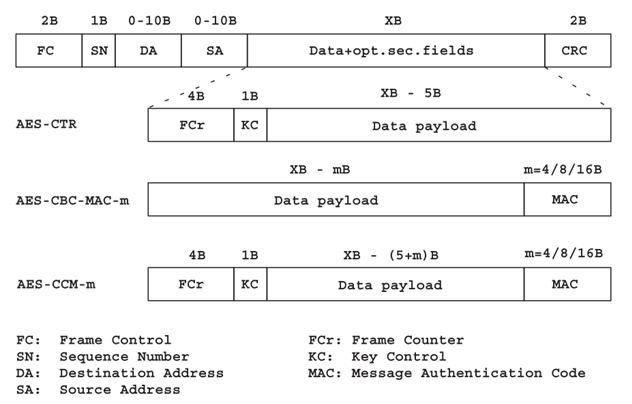
\includegraphics[scale = 0.7]{fig52.png}
	\caption{IEEE 802.15.4 frame with security header}
	\label{fig:Graph52}
\end{figure}

Các chế độ bảo mật được hỗ trợ bởi tiêu chuẩn 802.15.4 bao gồm tiêu chuẩn mã hóa nâng cao trong chế độ bộ đếm (AES-CTR) chỉ để mã hóa, AES trong chế độ chuỗi khối mật mã (AES-CBC) chỉ để xác thực tin nhắn và AES trong bộ đếm với CBC-MAC (AES- CCM), kết hợp mã hóa và xác thực tin nhắn. Đối với các chế độ MAC, mã xác thực được bao gồm là 4, 8 hoặc 16 byte. Bên cạnh chế độ null (các tính năng bảo mật bị tắt), AES-CCM là chế độ duy nhất được tiêu chuẩn yêu cầu, phải có sẵn trên tất cả các thiết bị tuân thủ tiêu chuẩn. Nó đã được chỉ ra rằng bộ bảo mật với mã hóa, AES-CTR, không nên được sử dụng riêng. Các mạng chỉ có mã hóa và không có xác thực dễ bị chèn các gói tin sai và đã được chứng minh là dễ bị tấn công. \\

Tiêu chuẩn IEEE 802.15.4 hiện đang sử dụng các khóa chia sẻ trước để mã hóa và xác minh tính toàn vẹn. \\

Triển khai bảo mật lớp liên kết IEEE 802.15.4 hỗ trợ xây dựng tiêu đề cho tất cả các chế độ bảo mật được mô tả trong tiêu chuẩn. Việc xây dựng khung 802.15.4 được thực hiện trong phần mềm, trong khi các hoạt động mật mã được thực hiện bởi chip RF. Phân phối khóa thủ công được sử dụng vì quản lý khóa không được chuẩn hóa trong 802.15.4. Do đó, một khóa xác định trước được sử dụng trên tất cả các nút trong mạng. \\

Bảo mật lớp liên kết IEEE 802.15.4 được áp dụng sau khi bản tin được nén và phân mảnh ở lớp 6LoWPAN. Điều quan trọng cần lưu ý là khi phân mảnh là cần thiết và bảo mật lớp liên kết được bật, tiêu đề bảo mật và / hoặc message integrity code  (MIC) được thêm vào mỗi phân mảnh. Do đó, khi tải trọng tăng lên, chi phí của các tiêu đề bảo mật lớp liên kết cũng tăng theo. 

\subsection{Bảo mật trong giao thức MQTT}
Bảo mật trong MQTT được chia thành nhiều lớp. Mỗi lớp ngăn chặn các loại tấn công khác nhau. Mục tiêu của MQTT là cung cấp một giao thức truyền thông nhẹ và dễ sử dụng cho Internet of Things. Bản thân giao thức chỉ xác định một số cơ chế bảo mật. Việc triển khai MQTT thường sử dụng các tiêu chuẩn bảo mật hiện đại khác.
\subsubsection{Xác thực MQTT với username/password}
Giao thức MQTT cung cấp các trường username và password trong thông báo CONNECT để xác thực. Máy khách có tùy chọn gửi tên người dùng và mật khẩu khi nó kết nối với nhà môi giới MQTT.

\begin{figure}[h]
	\centering
	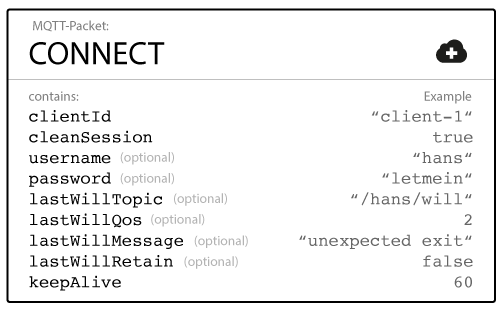
\includegraphics[scale = 0.7]{fig53.png}
	\caption{MQTT-Packet: CONNECT}
	\label{fig:Graph53}
\end{figure}

Username là một chuỗi được mã hóa UTF-8. Password là dữ liệu nhị phân với tối đa 65535 byte. Đặc tả MQTT nói rằng bạn có thể gửi username mà không có password, nhưng không thể gửi password mà không có username. MQTT phiên bản 3.1.1 cũng loại bỏ khuyến nghị trước đó cho mật khẩu 12 ký tự. \\

Khi bạn sử dụng xác thực username/password MQTT được tích hợp sẵn, Broker MQTT đánh giá thông tin đăng nhập dựa trên cơ chế xác thực được triển khai và trả về một trong các mã trả lại sau: 
\begin{table}[h]
	\centering
	\label{tab:tb2}
	\begin{tabular}{|c|c|}
		\hline
		Return Code & Return Code Response                                     \\ \hline
		0           & Kết nối được chấp nhận                                   \\ \hline
		4           & Kết nối bị từ chối, user name hoặc password không hợp lệ \\ \hline
		5           & Kết nối bị từ chối, không được phép                      \\ \hline
	\end{tabular}
	\caption{Bảng Return Code}
\end{table}
\subsubsection{TLS/SSL}
\noindent
\textbf{TLS là gì?} \\

Bảo mật lớp truyền tải (TLS) và lớp cổng bảo mật (SSL) cung cấp một kênh giao tiếp an toàn giữa máy khách và máy chủ. Về cốt lõi, TLS và SSL là các giao thức mật mã sử dụng cơ chế bắt tay để thương lượng các tham số khác nhau nhằm tạo kết nối an toàn giữa máy khách và máy chủ. Sau khi bắt tay hoàn tất, giao tiếp được mã hóa giữa máy khách và máy chủ được thiết lập và không kẻ tấn công nào có thể nghe trộm bất kỳ phần nào của giao tiếp. Máy chủ cung cấp chứng chỉ X509 (thường được cấp bởi cơ quan đáng tin cậy) mà máy khách sử dụng để xác minh danh tính của máy chủ. \\

\noindent
\textbf{Tại sao TLS lại quan trọng?} \\

Hãy tưởng tượng rằng bạn đang gửi một tấm bưu thiếp. Rõ ràng người nhận thẻ là ai và người đưa thư sẽ đảm bảo rằng thẻ sẽ đến. Nhưng, không có gì ngăn cản người đưa thư đọc nội dung của tấm thiệp. Trên thực tế, tất cả những ai tham gia vào việc chuyển phát bưu thiếp đều có thể đọc nội dung bưu thiếp của bạn. Một nhân viên bưu điện độc hại thậm chí có thể thay đổi nội dung thẻ của bạn!\\

Bản chất của kịch bản này cũng đúng đối với mạng máy tính nói chung và Internet nói riêng. Sử dụng TCP / IP thuần túy giống như gửi bưu thiếp. Gói TCP đi qua nhiều thành phần cơ sở hạ tầng (bộ định tuyến, tường lửa, Điểm trao đổi Internet) trước khi nó đến mục tiêu. Mọi người tham gia trên đường đi đều có thể đọc nội dung của gói tin bằng văn bản rõ ràng (và thậm chí sửa đổi nó). Đây không phải là một kịch bản hư cấu, lịch sử gần đây cho thấy lưu lượng Internet thường xuyên bị các cơ quan tình báo nghe lén. Mặc dù hầu hết những kẻ tấn công không có nhiều tài nguyên để nghe trộm kết nối của bạn, nhưng không khó để những kẻ tấn công tinh vi thực hiện các cuộc tấn công giữa hai người.\\

TLS là tất cả về việc cung cấp một kênh giao tiếp an toàn. TLS đảm bảo rằng nội dung giao tiếp của bạn không thể bị đọc hoặc thay đổi bởi các bên thứ ba. \\

\noindent
\textbf{MQTT và TLS} \\

MQTT dựa trên giao thức truyền tải TCP. Theo mặc định, các kết nối TCP không sử dụng giao tiếp được mã hóa. Để mã hóa toàn bộ giao tiếp MQTT, nhiều nhà môi giới MQTT (chẳng hạn như HiveMQ) cho phép sử dụng TLS thay vì TCP đơn thuần. Nếu sử dụng trường username và password của gói MQTT CONNECT cho cơ chế xác thực và ủy quyền  thì nên cân nhắc sử dụng TLS. \\

Cổng 8883 được tiêu chuẩn hóa cho kết nối MQTT bảo mật. Tên được chuẩn hóa tại IANA là “secure-mqtt”. Cổng 8883 được dành riêng cho MQTT qua TLS.

\newpage
\chapter{Thiết kế và thực hiện phần cứng}
\section{Tổng quan hệ thống}
Với mục tiêu triển khai hệ thống hệ thống giám sát chỉ số sinh tồn sử dụng mạng
6LowPAN và giao thức MQTT, em đã triển khai hệ thống gồm 4 khối: (1) Khối cảm biến, (2)
Khối border-router/gateway, (3) Khối server, (4) Khối ứng dụng giám sát.
\begin{figure}[h]
	\centering
	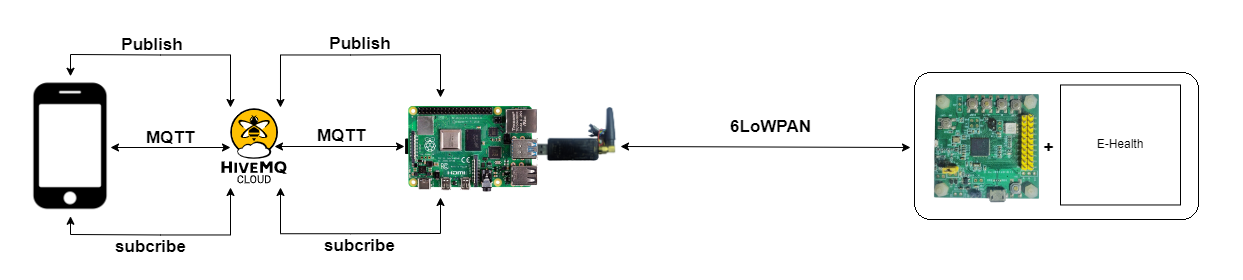
\includegraphics[scale = 0.5]{fig33.png}
	\caption{Sơ đồ tổng quan hệ thống}
	\label{fig:Graph33}
\end{figure}

\textbf{Khối cảm biến:} sử dụng board E-Health bao gồm các cảm biến SpO2, huyết áp, nhịp tim và nhiệt độ để đo các chỉ số sinh tồn rồi chuyển dữ liệu đo được đến board CC2538 thông qua UART sau đó gửi đến Border-router/gateway thông qua mạng 6LoWPAN. \\

\textbf{Khối border-router/gateway:} Border-router/gateway là nơi trung gian trong hệ thống mạng, nó kết nối mạng 6LoWPAN và mạng Internet, bao gồm Raspberry pi kết nối với một 6LoWPAN CC2538 USB DONGLE
(nhiệm vụ border router) qua đường serial UART hoặc USB. Raspberry được xem là gateway cũng như database/webserver của hệ thống, chịu trách nhiệm giao tiếp với 6LoWPAN border router qua đường serial UART, ngoài ra kết nối với mạng WLAN trong nhà qua chuẩn wifi để giao tiếp với các thiết bị không dây điện thoại, nhận lệnh điều khiển và xuất dữ liệu qua giao diện User Interface. 6LoWPAN
Border router đóng vai trò thu phát và chạy các giao thức của mạng 6LoWPAN giao tiếp với
Khối 6Lo-Server qua chuẩn 6LoWPAN/IPv6. \\

\textbf{Khối sever:} Sử dụng cloud server chạy MQTT broker là HiveMQ với chức năng
truyền tải thông tin giữa khối border-router và khối cảm biến thông qua giao
tiếp wifi nhằm mục đich điều khiển và giám sát các chỉ số sinh tồn từ xa. \\

\textbf{Khối ứng dụng giám sát} là một ứng dụng Android có các chức năng chính như:
\begin{itemize}
	\item Nhận các thông số sinh tồn được gửi từ khối border-router/gateway thông qua cloud HiveMQ hiện thị cho người dùng.
	\item Vẽ đồ thị theo thời gian các chỉ số nhiệt độ, SpO2 và nhịp tim.
	\item Hiển thị các chuẩn giá trị tham chiếu để người dùng có thể so sánh với các thông số sinh tồn đo được để sử trí kịp thời. 
	\item Lưu lịch sử đo huyết áp gần nhất
\end{itemize}
\section{Chi tiết các sensors và phần cứng liên quan}
\subsection{Module CC2538}
Board mạch phát triển từ module C2538. CC2538 là module Contiki 6LoWPAN được sản
xuất bởi hãng TI (Texas Instruments). Module này nhanh chóng được trở nên phổ biến trong
các ứng dụng IOT (Internet of thing).
\begin{figure}[h]
	\centering
	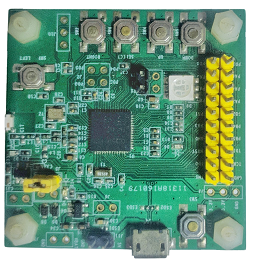
\includegraphics[scale = 0.7]{fig34.png}
	\caption{Module TI SoC CC2538}
	\label{fig:Graph34}
\end{figure}

Vi điều khiển: Chip ARM Cortex-M3 R mạnh mẽ, tốc độ clock lên đến 32-MHz, flash nội
512KB, hỗ trợ update firmware từ xa trên chip, RAM 32 KB, hỗ trợ debug thông qua jTAG
và cJTAG cũng như hỗ trợ nạp firmware thông qua bootloader. \\


Thông số RF: Bộ thu phát RF hoạt động ở tần số 2.4-GHz theo chuẩn 802.15.4, độ nhạy
máy thu -97 dBm, công suất phát lên đến 7 dBm. \\

Công suất thấp: Active-Mode RX (CPU Idle): 20 mA, active-Mode TX tại 0 dBm (CPU Idle):
24 mA, Power Mode 1 (Chế độ ngủ 4-us, duy trì 32-KB RAM, full thanh ghi): 0.6 mA, Power
Mode 2 (Chế độ ngủ định kì, duy trì 16-KB RAM, hiệu chỉnh thanh ghi): 1.3 $\mu$A, Power Mode
3 (Ngắt ngoài, duy trì 16-KB RAM, hiệu chỉnh thanh ghi): 0.4 $\mu$A, dải điện áp hoạt động rộng:
2V - 3.6V. \\

Ngoại vị: $\mu$DMA, 4 x Timer dùng chung (32-bit hoặc 2 x 16-Bit), 32-Bit 32kHz sleep Timer,
12-Bit ADC với 8 kênh và độ chia có thể điều chỉnh, cảm biến nguồn và nhiệt độ on chip, 2 x SPI, 2 x UART, I2C, 32 GPIO (28 x 4 mA, 4 x 20 mA), Watchdog Timer. \\


C2538 có tài nguyên khá lớn. SoC này có 512 KB Flash và 32 KB RAM, khá hào phóng
trong phân khúc nhúng giá rẻ. Hiện nay SoC CC2538 đang dược cộng đồng hỗ trợ rất tốt Contiki OS,
nó dang được tích cực phát triển bởi cộng đồng develop khắp nơi trên thế giới. Nạp chương
trình qua cổng serial với backdoor bootloader enable. Ngoài ra còn có tính năng Over the air
update. Đây là đặt tính khá quan trọng khi làm việc với mạng mesh có khoảng vài chục đến
vài trăm node trong mạng, firmware cần cập nhật, và các node không cần cắm vào PC để nạp
tuần tự. Điều này có được nhờ vào tài nguyên flash khá lớn, có thể đẩy được đến 3 image vào
trong flash. 
\begin{figure}[h]
	\centering
	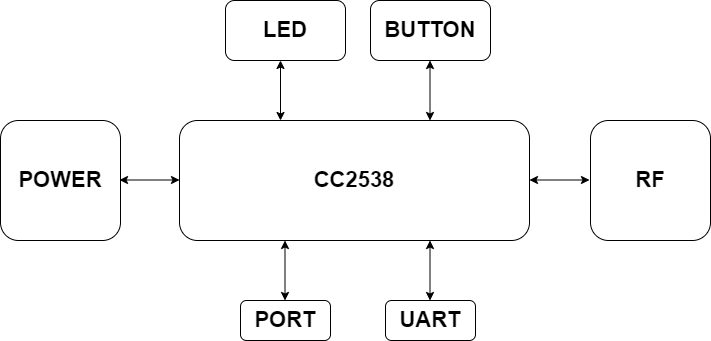
\includegraphics[scale = 0.4]{fig35.png}
	\caption{Sơ đồ khối CC2538 Development Kit.}
	\label{fig:Graph35}
\end{figure}

Mô tả các khối trong sơ đồ khối: 
\begin{itemize}
	\item CC2538: Đây là MCU chính sử dụng trên board, khối này chính là module CC2538
	\item Power: Nguồn 5V, nguồn micro USB, hoặc nguồn Pin 3.7V
	\item RF: Đây là khối anten sử dụng để giao tiếp không dây, sử dụng PCB anten
	\item UART: khối này là giao tiếp UART, qua đó để debug, giao tiếp serial và nạp firmware thông với chế độ bootloader.
	\item PORT: Mở rộng kết nối cho board, để giao tiếp với các thiết bị khác
	\item Button, LED: bao gồm nút reset, đèn báo nguồn, các button, LED cho người sử dụng tùy chon chức năng
\end{itemize}
\newpage
\begin{figure}[h]
	\centering
	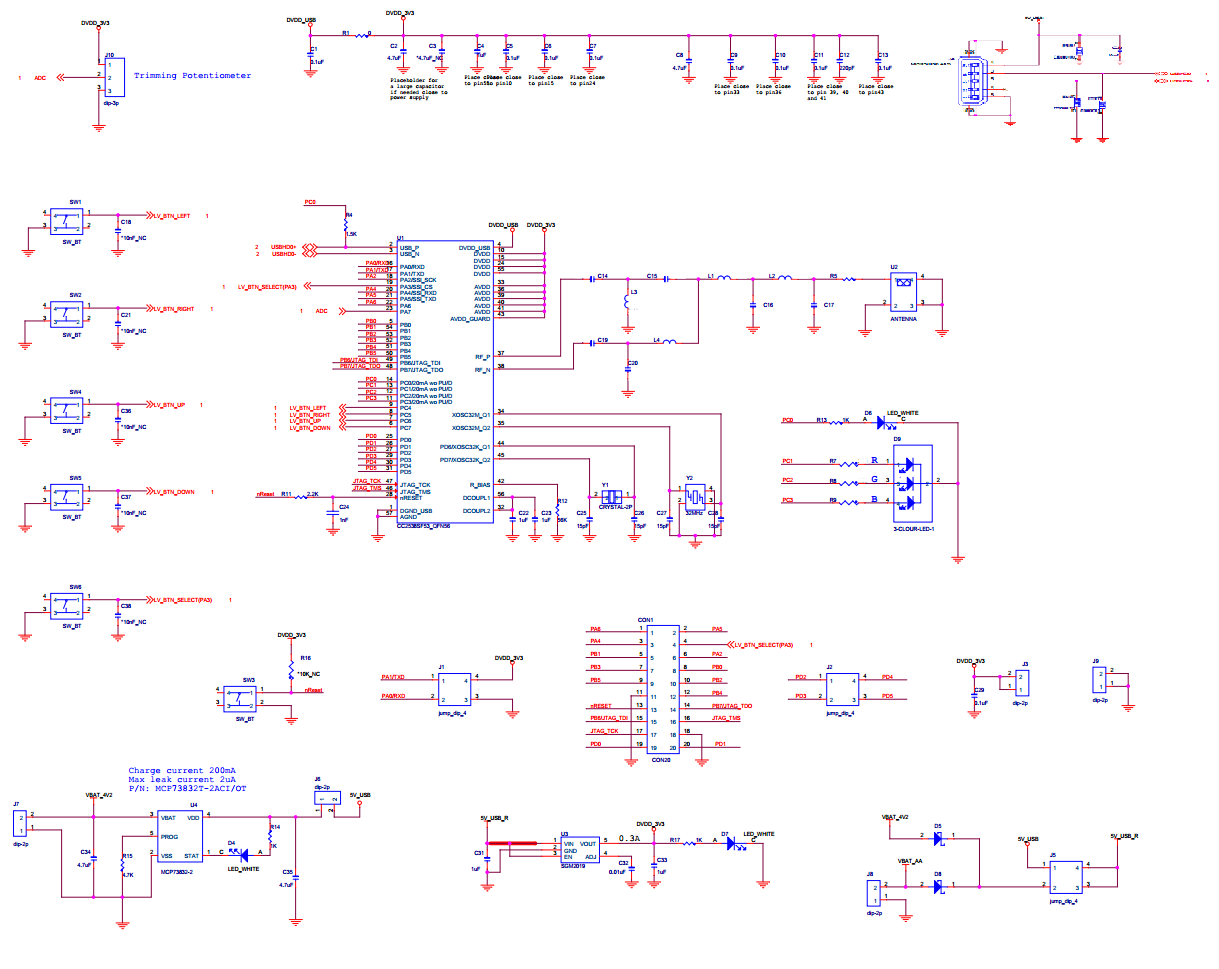
\includegraphics[scale = 0.5]{fig36.png}
	\caption{Schematic CC2538 Development Kit}
	\label{fig:Graph36}
\end{figure}


\subsection{CC2538 usb dongle}
\begin{figure}[h]
	\centering
	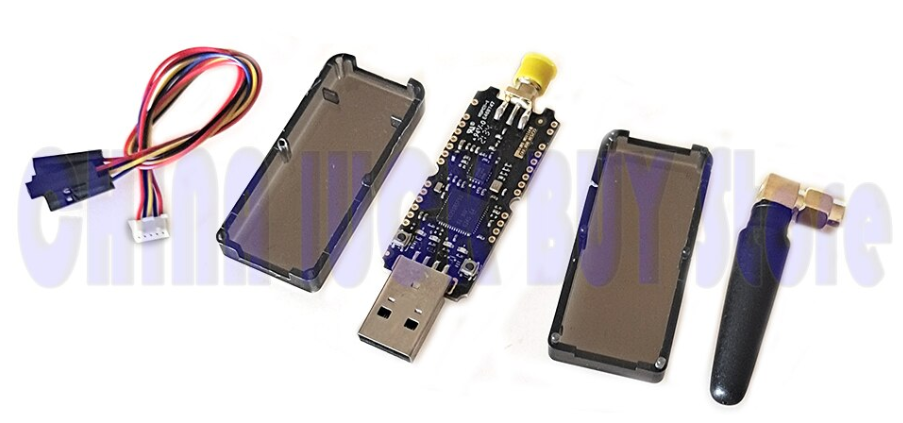
\includegraphics[scale = 0.24]{fig37.png}
	\caption{CC2538 usb dongle}
	\label{fig:Graph37}
\end{figure}
CC2538 usb dongle có tính năng tương tự như module CC2538 nhưng có thêm bộ phận USB để giao tiếp với raspberry pi và sử dụng anten ngoài thay vì anten PCB như module CC2538.
\newpage
\begin{figure}[h]
	\centering
	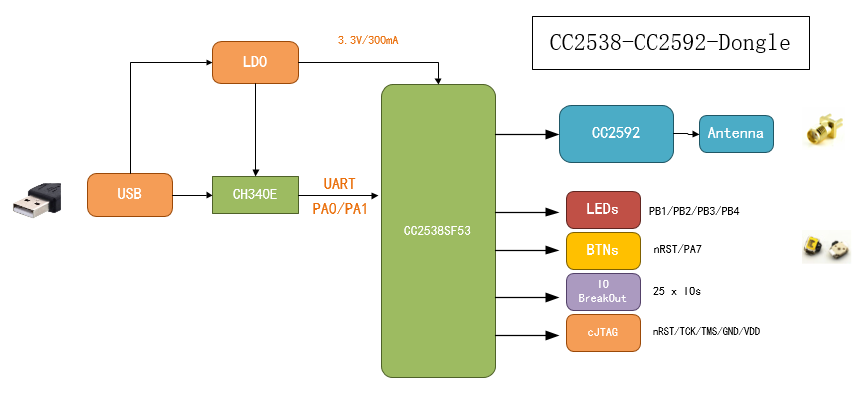
\includegraphics[scale = 0.5]{fig38.png}
	\caption{Sơ đồ khối CC2538 usb dongle}
	\label{fig:Graph38}
\end{figure}
Tính năng:
\begin{itemize}
	\item 2.4GHz multiprotocol RF development board(OpenThread,Zigbee,BLE,IEEE802.15.4,6LoWPAN based on TI CC2538SF53 + CC2592 chip
	\item Giao tiếp với máy tính thông qua cầu nối USB-UART CH340E chung
	\item cJTAG debug header, flashed firmware hoặc debug bằng JTAG
	\item Tự lập trình thông qua TI serial bootloader với bootloader bit được bật
	\item Cổng ăng-ten SMA cho ăng-ten bên ngoài
	\item 4xLED (PB1 / PB2 / PB3 / PB4)
	\item 2xButtons (BTN1 - PA7 <Bootloader-enable> RST - nRESET)
	\item IO với lỗ 2.0mm để kết nối thiết bị ngoại vi
	\item LDO công suất thấp
	\item Bảo vệ ESD với giao diện USB
	\item Tương thích với CC2538 + CC2592 SmartRF06EVB từ TI
\end{itemize}
\subsection{Raspberry pi 4}
Raspberry Pi 4 Model B là sản phẩm mới nhất trong dòng máy tính Raspberry Pi phổ biến. Nó cung cấp sự gia tăng đột phá về tốc độ bộ xử lý, hiệu suất đa phương tiện, bộ nhớ và kết nối so với Raspberry Pi 3 Model B + thế hệ trước, trong khi vẫn giữ được khả năng tương thích ngược và mức tiêu thụ điện năng tương tự. Đối với người dùng cuối, Raspberry Pi 4 Model B cung cấp hiệu suất máy tính để bàn tương đương với các hệ thống PC x86 cấp thấp. \\

Các tính năng chính của sản phẩm này bao gồm bộ vi xử lý lõi tứ 64-bit hiệu suất cao, hỗ trợ hiển thị kép ở độ phân giải lên đến 4K thông qua một cặp cổng micro-HDMI, giải mã video phần cứng lên đến 4Kp60, RAM lên đến 8GB, kép. - LAN không dây băng tần 2.4 / 5.0 GHz, Bluetooth 5.0, Gigabit Ethernet, USB 3.0 và khả năng PoE (thông qua tiện ích bổ sung PoE HAT riêng biệt). \\

Mạng LAN không dây băng tần kép và Bluetooth có chứng nhận tuân thủ theo mô-đun, cho phép bo mạch được thiết kế thành các sản phẩm cuối với việc kiểm tra tuân thủ giảm đáng kể, cải thiện cả chi phí và thời gian đưa ra thị trường. 
\begin{figure}[h]
	\centering
	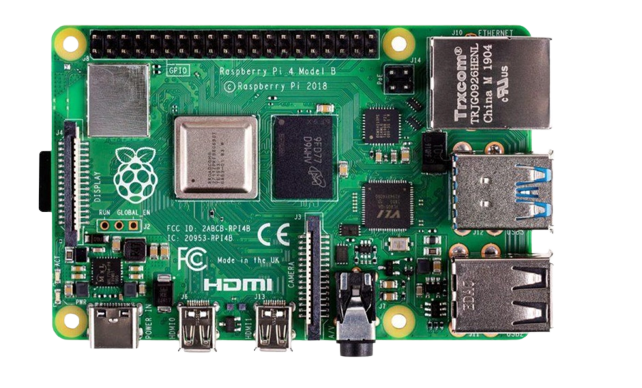
\includegraphics[scale = 0.5]{fig39.png}
	\caption{Raspberry pi 4}
	\label{fig:Graph39}
\end{figure}

\textbf{Đặc điểm kỹ thuật:}
\begin{itemize}
	\item Phần cứng:
		\begin{description}
		\item[-] Lõi tứ 64-bit ARM-Cortex A72 chạy ở tốc độ 1,5 GHz
		\item[-] Tùy chọn RAM 1, 2 và 4 Gigabyte LPDDR4
		\item[-] Giải mã phần cứng H.265 (HEVC) (lên đến 4Kp60)
		\item[-] Giải mã phần cứng H.264 (lên đến 1080p60)
		\item[-] Đồ họa 3D VideoCore VI
		\item[-] Hỗ trợ đầu ra hiển thị HDMI kép lên đến 4Kp60
		\end{description}
	\item Giao diện:
		\begin{description}
		\item[-] 802.11 b/g/n/ac Wireless LAN
		\item[-] Bluetooth 5.0 với BLE
		\item[-] 1x SD Card
		\item[-] 2x cổng micro-HDMI hỗ trợ màn hình kép lên đến độ phân giải 4Kp60
		\item[-] 2x USB2 ports
		\item[-] 2x USB3 ports
		\item[-] 1x cổng Gigabit Ethernet (hỗ trợ PoE với PoE HAT bổ sung)
		\item[-] 1 cổng máy ảnh Raspberry Pi (MIPI CSI 2 làn)
		\item[-] 1x Cổng hiển thị Raspberry Pi (MIPI DSI 2 làn)
		\item[-] 28x người dùng GPIO hỗ trợ các tùy chọn giao diện khác nhau:
			\begin{description}
				\item[+] 6x UART
				\item[+] 6x I2C
				\item[+] 5x SPI
				\item[+] 1x SDIO interface
				\item[+] 1x DPI (Parallel RGB Display)
				\item[+] 1x PCM, 2x PWM channels
				\item[+] 3x GPCLK outputs
			\end{description}
		\end{description}
\end{itemize}
\subsection{Board E-Health}
\begin{figure}[h]
	\centering
	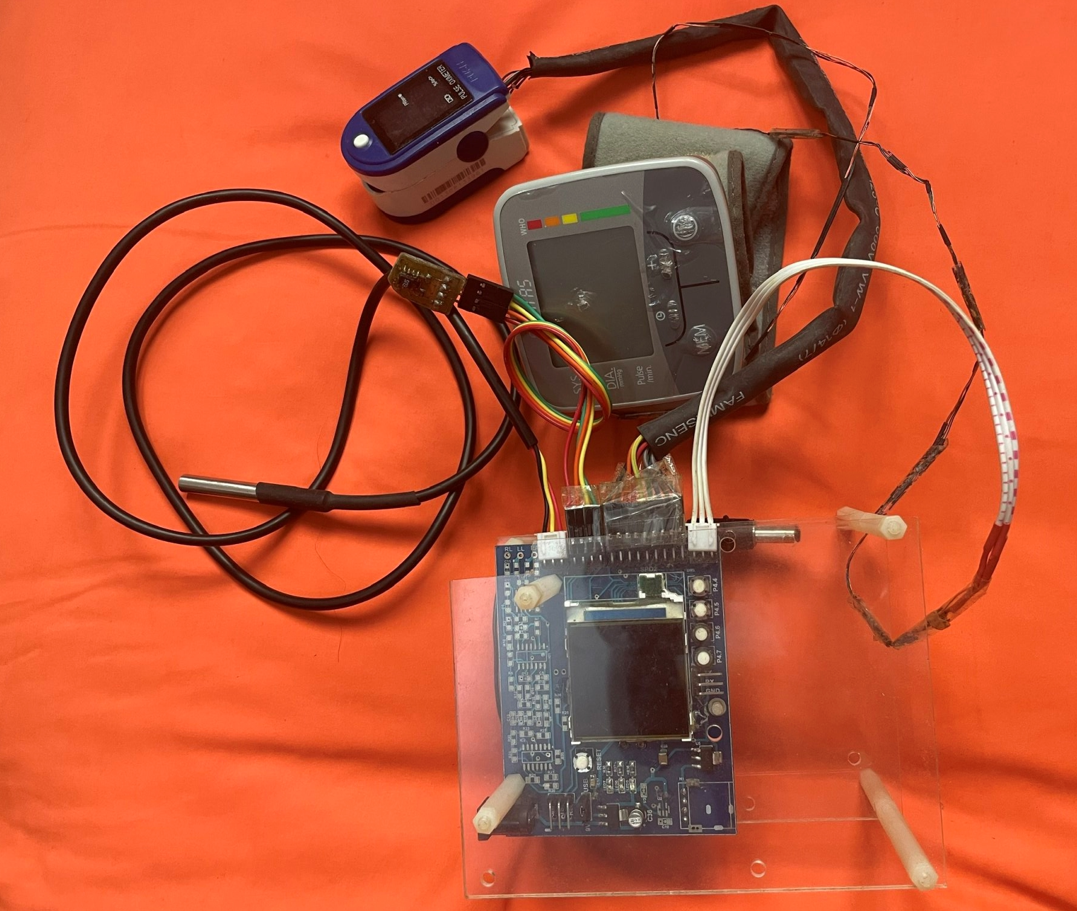
\includegraphics[scale = 0.4]{fig40.png}
	\caption{Board E-Health}
	\label{fig:Graph40}
\end{figure}

Máy đo E-Health sử dụng vi điều khiển MSP430F6659 làm trung tâm xử lý. Để đo các
tín hiệu y khoa, máy đo E-Health kết nối với các thiết bị như cảm biến nhiệt độ DS18B20, máy đo SpO2, máy đo huyết áp SANITAS SBC27. Ngoài ra, một cảm biến nhiệt độ khác cũng được sử dụng để lấy nhiệt độ, đó là DS18B20. \\

Máy đo hiển thị trực tiếp số liệu đo được thông qua LCD và truyền kết quả tới server thông qua 2 chân UART. \\

Máy đo có thể sử dụng 2 nguồn là USB hoặc PIN (sử dụng 4 pin 1.5V), chuyển đổi nhanh chóng thông qua một Jump. 
\newpage
\begin{figure}[h]
	\centering
	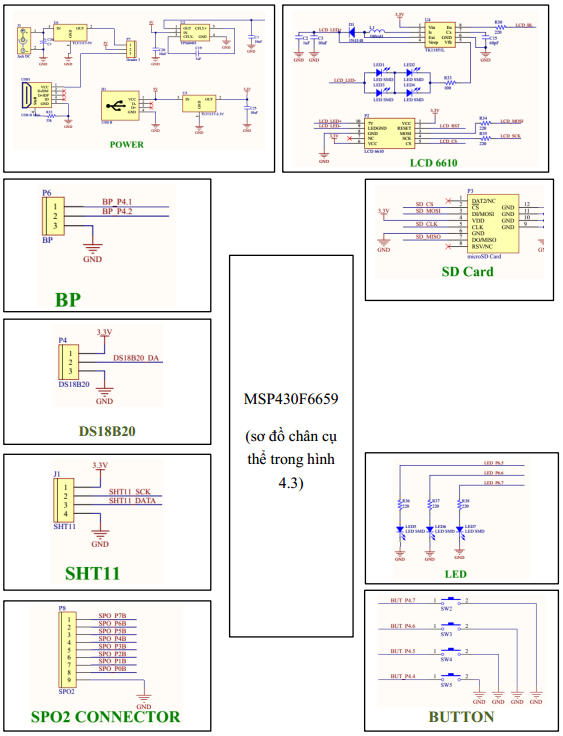
\includegraphics[scale = 0.85]{fig41.png}
	\caption{Sơ đồ thiết bị board E-Health}
	\label{fig:Graph41}
\end{figure}

\newpage
\begin{figure}[h]
	\centering
	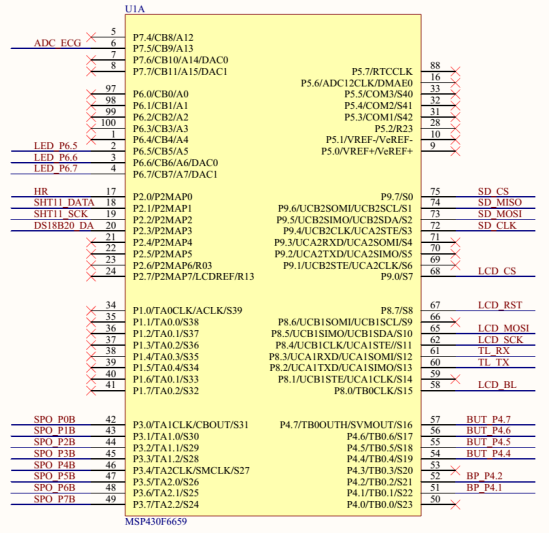
\includegraphics[scale = 0.9]{fig42.png}
	\caption{Sơ đồ chân nối với các thiết bị của vi điều khiển MSP430F6659}
	\label{fig:Graph42}
\end{figure}
\textbf{Sơ lược về vi điều khiển MSP430F6659} là một dòng vi điều khiển nổi tiếng của hãng Texas
Instruments. Với nhiều ưu điểm nổi bật, MSP430 được khá nhiều người sử dụng. Một số ưu
điểm của dòng MSP430 như sau:
\begin{itemize}
	\item Tiêu thụ năng lượng cực thấp
	\item Thiết kế nhỏ gọn
	\item Bộ xử lý hiện đại với các module tương tự và số
	\item Lập trình thay đổi code một cách linh hoạt
\end{itemize}
\newpage
\begin{figure}[h]
	\centering
	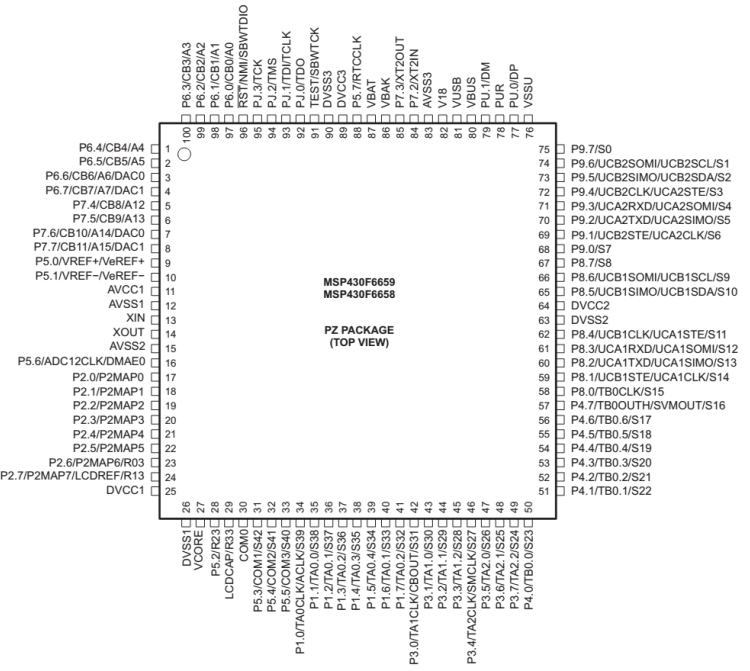
\includegraphics[scale = 0.5]{fig43.png}
	\caption{Sơ đồ chân MSP430F6659}
	\label{fig:Graph43}
\end{figure}

\textbf{Cảm biến nhiệt độ DS18B20} của hãng Dallas là cảm biến phổ biến để đo nhiệt độ. Cảm
biến này có nhiều ưu điểm nổi bật như gọn nhẹ, giá rẻ, bền, chống thấm nước.
\begin{figure}[h]
	\centering
	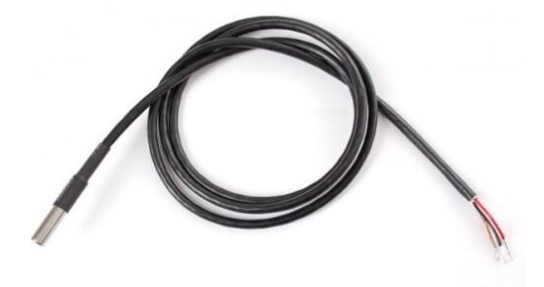
\includegraphics[scale = 0.5]{fig44.png}
	\caption{Cảm biến nhiệt độ DS18B20}
	\label{fig:Graph44}
\end{figure}

\textbf{Máy đo huyết áp SANITAS SBC27:} Máy đo này sử dụng Eeprom 24C08 giao tiếp theo theo chuẩn I2C để lưu dữ liệu nên để lấy được dữ liệu từ máy đo phải capture đường dữ liệu nối với Eeproom 24C08 của máy
đo bằng cách nối 2 dây SDA và SCL với P4.1 và P4.2 và chân GND nối chung với GND của vi điều khiển. Máy đo
được cấp nguồn riêng bên ngoài với 2 pin AAA 1.5V và cho kết quả đo sau 15 giây.
\newpage
\begin{figure}[h]
	\centering
	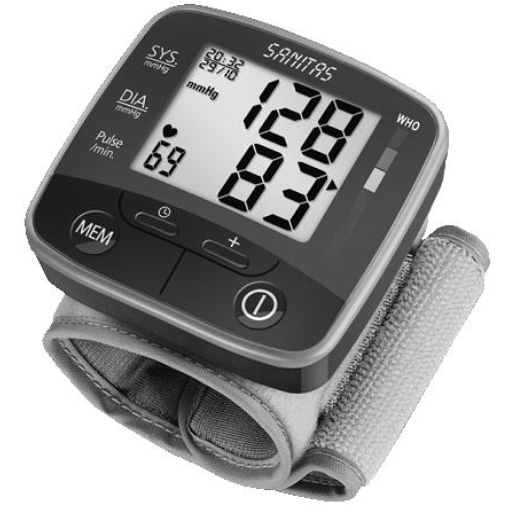
\includegraphics[scale = 0.4]{fig45.png}
	\caption{Máy đo huyết áp cổ tay SANITAS SBC27}
	\label{fig:Graph45}
\end{figure}
\textbf{Máy đo nhịp tim và nồng độ oxi trong máu SPO2:} Để đo nồng độ oxi trong máu và nhịp tim board E-Health sử dụng máy đo Pulse Oximeter CMS50DL. Một máy đo có kích thước nhỏ gọn, tiện lợi, có màn hình hiển thị Led.
\begin{figure}[h]
	\centering
	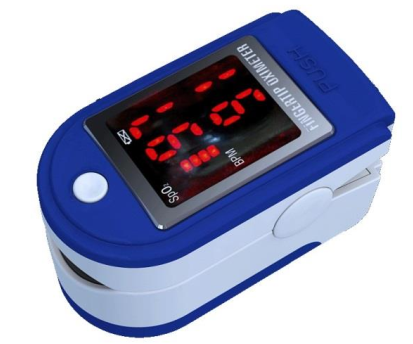
\includegraphics[scale = 0.5]{fig46.png}
	\caption{Máy đo Pulse Oximater}
	\label{fig:Graph46}
\end{figure}
\section{Thiết kế Firmware}
Firmware là chương trình chạy trên nút cảm biến và border-router kết nối với gateway. Trong
khi border-router đã có firmware chuẩn thì firmware tại các nút cảm biến cần phải thiết
kế để phục vụ mục đích, yêu cầu của ứng dụng. Ở phần thiết kế firmware này sẽ đề xuất một
Framework chung cho ứng dụng bao gồm qui định tất cả các lớp trong mạng 6LoWPAN sử
dụng chung duy nhất framework này. \\

Để đạt mục tiêu đề ra cũng như hướng đến việc sử dụng mạng lưới có khả năng mở rộng
cao, một Framework được đề xuất như sau. 
\newpage
\begin{figure}[h]
	\centering
	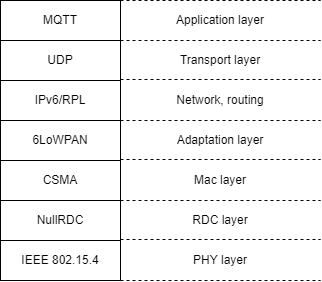
\includegraphics[scale = 0.7]{fig47.png}
	\caption{Framework của đề tài}
	\label{fig:Graph47}
\end{figure}

\textbf{Physical Layer:} Ở lớp Physical, để tránh va chạm và can nhiễu bởi các thiết bị không dây khác, đặc biệt là mạng Wifi ta cấu hình ở lớp Physical Layer với tần số phát ở kênh 26. \\

\textbf{RDC layer:} Ở lớp RDC ta cấu hính NullRDC để truyền thông không bao giờ tắt tín hiệu vô tuyến. \\

\textbf{MAC layer:} Ở lớp MAC ta dùng CSMA để có thể tránh xung đột khi truyền gói tin. Hạn chế mất gói
trong mạng (mặc dù đánh đổi thời gian trễ khi truyền gói tin). \\

\textbf{Transport Layer:} Với những ưu điểm đã được trình bày ở phần lý thuyết, việc áp dụng UDP là phù hợp nhất. \\

\textbf{Application Layer:} Sử dụng giao thức MQTT.
\chapter{Thiết kế và thực hiện phần mềm}
\section{Khối cảm biến}
Giải thuật xử lý tại khối cảm biến được mô tả tổng quan như trong Hình \ref{fig:Graph48}. CC2538 sẽ nhận data liên tục từ board E-Health rồi đưa lên mạng 6LoWPAN truyền đến border-router/gateway.
\begin{figure}[h]
	\centering
	\includegraphics[scale = 0.5]{fig48.png}
	\caption{Giải thuật thực hiện tại khối cảm biến}
	\label{fig:Graph48}
\end{figure}

Tất cả chương trình thực hiện ở khối cảm biến trên CC2538 Development Kit được tải lên tại đây: \url{https://github.com/vominhtribku/E-health}
\newpage
\section{Khối border-router/gateway}
\begin{figure}[h]
	\centering
	\includegraphics[scale = 0.5]{fig49.png}
	\caption{Sơ đồ tổng quát phần mềm khối Boder-router/gateway}
	\label{fig:Graph49}
\end{figure}

Phần mềm của hệ thống được viết và chạy trên máy tính nhúng Raspberry Pi, trong đó sẽ
thực hiện việc giao tiếp với cloud HiveMQ thông gia giao thức MQTT cũng như giao tiếp với Border Router Node CC2538DK để giao tiếp với mạng 6LoWPAN. Border Router program sẽ chạy công cụ tunslip6 được Contiki OS hỗ trợ để giao tiếp với mạng 6LoWPAN. \\

Chương trình Border-router thực hiện trên CC2538 USB DONGLE được tải lên tại đây: \url{https://github.com/vominhtribku/border-router-ehealth} \\

Chương trình giao tiếp với MQTT cloud thực hiện trên Raspberry Pi được tải lên tại đây: \url{https://github.com/vominhtribku/Gateway-rasp}



\subsection{Tunslip6}
Tunslip6 là tool được hỗ trợ trong Contiki OS, Tunslip6 là công cụ làm câu nối IPv6 traffic
với host, border router, thông qua serial. Tunslip6 tạo ra một virtual network interface (tun) ở
phía host và sử dụng SLIP (serial line internet protocol) để đóng gói và pass IP traflic thông
qua serial. Tun interface có thể được sử dụng như bất kì network interface thực tế nào: routing,
traffic forwarding, Wireshark analysis, vv.
\subsection{Hệ điều hành Raspbian}
Đây là hệ điều hành cơ bản, phổ biến nhất và do chính Raspberry Pi Foundation cung cấp.
Nó cũng được hãng khuyến cáo sử dụng, nhất là cho người mới bắt đầu làm quen với RPI.
\begin{figure}[h]
	\centering
	\includegraphics[scale = 0.5]{fig50.png}
	\caption{Hệ điều hành Raspbian}
	\label{fig:Graph50}
\end{figure}

Raspbian có dung lượng sau khi giải nén là khoảng gần 4GB, bạn cần tối thiểu 1 cái thẻ 4GB
để có thể sử dụng Raspbian. Tuy nhiên, Raspbian có phát hành phiên bản Raspbian Lite, với
dung lượng chỉ khoảng 400MB chuyên dùng cho các ứng dụng IOT không cần truy xuất màn
hình, phù hợp cho việc chọn làm Gateway. Theo đánh giá chung thì Raspbian Lite hoạt động
rất ổn định, tốc độ nhanh. 
\section{Khối ứng dụng}
\begin{figure}[h]
	\centering
	\includegraphics[scale = 0.5]{fig51.png}
	\label{fig:Graph51}
\end{figure}
\noindent
\textbf{Flutter là gì?} 
\begin{itemize}
	\item Flutter là mobile UI framework của Google để tạo ra các giao diện chất lượng cao trên iOS và Android trong khoảng thời gian ngắn. Flutter hoạt động với những code sẵn có được sử dụng bởi các lập trình viên, các tổ chức.
	\item Flutter hoàn toàn miễn phí và cũng là mã nguồn mở.
\end{itemize}
\noindent
\textbf{Đặc điểm nổi bật}
\begin{itemize}
	\item Fast Development: Tíng năng Hot Reload hoạt động trong milliseconds để hiện thị giao diện tới bạn. Sử dụng tập hợp các widget có thể customizable để xây dựng giao diện trong vài phút. Ngoài ra Hot Reload còn giúp bạn thêm các tính năng, fix bug tiết kiệm thời gian hơn mà không cần phải thông qua máy ảo, máy android hoặc iOS.
	\item Expressive and Flexible UI: Có rất nhiều các thành phần để xây dựng giao diện của Flutter vô cùng đẹp mắt theo phong cách Material Design và Cupertino, hỗ trợ nhiều các APIs chuyển động, smooth scrolling...
	\item Native Performance: Các widget của fluter kết hợp các sự khác biệt của các nền tảng ví dụ như scrolling, navigation, icons, font để cung cấp một hiệu năng tốt nhất tới iOS và Android.
\end{itemize}
\noindent
\textbf{Tại sao nên sử dụng Flutter ?}
\begin{itemize}
	\item Nếu bạn đang tìm kiếm các phương pháp thay thế để phát triển ứng dụng Android, bạn nên cân nhắc thử Flutter của Google, một framework dựa trên ngôn ngữ lập trình Dart. Dart là một static type language nên nó là AOT (Ahead of Time). Trong khi đó nó cũng là JIT (Just in Time) giống như các dynamic type language. Khi dev thì nó sử dụng JIT để hỗ trợ Hot Load và build release thì dùng AOT để tối ưu hiệu năng như một native code bình thường.
	\item Phát triển ứng dụng nhanh chóng: Tính năng hot reload của nó giúp bạn nhanh chóng và dễ dàng thử nghiệm, xây dựng giao diện người dùng, thêm tính năng và sửa lỗi nhanh hơn. Trải nghiệm tải lại lần thứ hai, mà không làm mất trạng thái, trên emulator, simulator và device cho iOS và Android.
	\item UI đẹp và biểu cảm: Thỏa mãn người dùng của bạn với các widget built-in đẹp mắt theo Material Design và Cupertino (iOS-flavor), các API chuyển động phong phú, scroll tự nhiên mượt mà và tự nhận thức được nền tảng.
	\item Truy cập các tính năng và SDK native: Làm cho ứng dụng của bạn trở nên sống động với API của platform, SDK của bên thứ ba và native code. Nó cho phép bạn sử dụng lại mã Java, Swift và ObjC hiện tại của mình và truy cập các tính năng và SDK native trên iOS và Android.
	\item Phát triển ứng dụng thống nhất: Flutter có các công cụ và thư viện để giúp bạn dễ dàng đưa ý tưởng của mình vào cuộc sống trên iOS và Android. Nếu bạn chưa có kinh nghiệm phát triển trên thiết bị di động, thì Flutter là một cách dễ dàng và nhanh chóng để xây dựng các ứng dụng di động tuyệt đẹp. Nếu bạn là một nhà phát triển iOS hoặc Android có kinh nghiệm, bạn có thể sử dụng Flutter cho các View của bạn và tận dụng nhiều code Java / Kotlin / ObjC / Swift hiện có của bạn.
\end{itemize}

Ở khối ứng dụng em thiết một chương trình app chạy trên điện thoại dựa trên flutter để đọc dữ liệu từ cloud MQTT mà gateway gửi lên. Ứng dụng có chức năng chính như:
\begin{itemize}
	\item Nhận các thông số sinh tồn được gửi từ khối border-router/gateway thông qua cloud HiveMQ hiện thị cho người dùng.
	\item Vẽ đồ thị theo thời gian các chỉ số nhiệt độ, SpO2 và nhịp tim.
	\item Hiển thị các chuẩn giá trị tham chiếu để người dùng có thể so sánh với các thông số sinh tồn đo được để sử trí kịp thời. 
	\item Lưu lịch sử đo huyết áp gần nhất.
\end{itemize}

Toàn bộ source code của App được tải lên tại đây: \url{https://github.com/vominhtribku/MQTT-Flutter-App}

\section{Bảo mật}
Đối với thiết kế bảo mật hệ thống trong ứng dụng này, tôi sẽ kết hợp việc áp dụng
tổng thể cơ chế bảo mật ở nhiều mức độ:
\begin{enumerate}
	\item Yếu tố an ninh cần thiết cho sự toàn vẹn dữ liệu dựa trên mật khẩu. Thiết lập
	mật khẩu cho kết nối giữa các máy khách MQTT và Broker HiveMQ.
	\item Cơ chế bảo mật ở tầng vận chuyển TLS để truy cập Broker HiveMQ
	bảo mật SSL từ thiết bị Android.
	\item Sử dụng cơ chế bảo mật Link Layer Security. Sử dụng mã hoá để cung cấp tính bảo mật
	và toàn vẹn dữ liệu cho bản tin. Các mục tiêu an ninh chỉ có thể được đáp ứng
	bằng cách bảo vệ cuộc đối thoại giữa hai nút đầu cuối. Cuộc đối thoại giữa hai
	lớp đầu cuối do đó được đáp ứng tốt nhất bằng cách mã hoá. Và tôi sẽ sử dụng
	LLSEC driver của Contiki để mã hoá kết nối giữa hai nút đầu cuối trong mạng
	6LoWPAN. LLSEC cho phép mã hoá và xác thực tất cả các gói tin trao đổi trên
	phương tiện WSN sử dụng mức độ mã hoá cao nhất AES-128. Không giống như
	việc phản ứng với các lỗ hổng bảo mật của IEEE 802.11, IEEE 802.15.4 yêu cầu
	sự hỗ trợ của các cơ chế mã hoá khá mạnh từ mỗi nút mạng, một yêu cầu mà hầu
	hết các chip IEEE 802.15.4 hiện nay có thể đáp ứng được. Cơ chế mã hoá được
	dựa trên thuật toán mã hoá AES hiện đại, được cộng đồng quốc tế lựa chọn thay
	thế cho thuật toán DES đã lỗi thời. IEEE 802.15.4 sử dụng AES trong bộ đếm
	với chế độ CBC-MAC, cung cấp không chỉ cơ chế mã hoá mà còn
	cả kiểm tra tính toán vẹn dữ liệu. \\
	\begin{table}[h]
		\centering
		\label{tab:tb3}
		\begin{tabular}{|c|c|c|}
			\hline
			\textbf{Giá trị} & \textbf{Mức bảo mật} & \textbf{Ý nghĩa}                             \\ \hline
			0x00             & NO\_SECURITY          & Không bảo mật. Không mã hoá. Không xác thực. \\ \hline
			0x01             & AES\_CBC\_MAC\_32       & 4-byte MIC. Không mã hoá. Có xác thực.       \\ \hline
			0x02             & AES\_CBC\_MAC\_64       & 8-byte MIC. Không mã hoá. Có xác thực.       \\ \hline
			0x03             & AES\_CBC\_MAC\_128      & 16-byte MIC. Không mã hoá. Có xác thực.      \\ \hline
			0x04             & AES\_CTR              & Có mã hoá dữ liệu. Không xác thực dữ liệu.   \\ \hline
			0x05             & AES\_CCM\_32           & 4-byte MIC. Có mã hoá. Có xác thực           \\ \hline
			0x06             & AES\_CCM\_64           & 8-byte MIC. Có mã hoá. Có xác thực           \\ \hline
			0x07             & AES\_CCM\_128          & 16-byte MIC. Có mã hoá. Có xác thực          \\ \hline
		\end{tabular}
		\caption{Các mức bảo mật LLSEC}
	\end{table}
\end{enumerate}

\newpage
\chapter{Kết quả thực hiện}
\section{Kết quả truyền nhận trong mạng 6LoWPAN}
\begin{figure}[h]
	\centering
	\includegraphics[scale = 0.5]{fig65.png}
	\caption{Topology của mạng 6LoWPAN sử dụng trong đề tài}
	\label{fig:Graph65}
\end{figure}
Địa điểm thực hiện là ở phòng ở của Ký túc xá Đại Học Bách Khoa TP.HCM. Anten
được bố trí sao cho thân anten vuông góc với mặt đất. Thực hiện tổng cộng là 2 node
với 1 node là border roter, node còn lại là client. Node là border router sẽ thực hiện đo đạc đánh giá hiệu suất truyền bằng cách ping tới node client với mỗi khoảng thời gian là 1 giây. \\

Đặt border-router ở độ cao 0.7m, end-node ở độ cao 0.5m và khoảng cách giữa border-router và end-node là 3m ta được kết quả truyền nhận như hình \ref{fig:Graph64}.
\begin{figure}[h]
	\centering
	\includegraphics[scale = 0.7]{fig64.png}
	\caption{Kết quả truyền nhận trong mạng}
	\label{fig:Graph64}
\end{figure}

Số gói end-node truyền là 481, số gói border-router nhận là 481. Do đó tỷ lệ truyền thành công gói tin từ end-node đến border-router là 100\%. Vì ứng dụng của đề tài nằm trong phạm vi diện tích hẹp nên mạng 6LoWPAN có thể đáp ứng được hoàn toàn yêu cầu, tín hiệu sẽ được truyền tải liên tục mà không bị mất hay bị gián đoạn.


\section{Kết quả phần cứng}
\subsection{Khối cảm biến}
Khối cảm biến bao gồm CC2538 Development Kit và board E-Health gồm các cảm biến huyết áp, nhịp tim và SpO2 được kết nối với nhau qua giao tiếp UART. hình ảnh chi tiết xem hình \ref{fig:Graph54}.
\begin{figure}[h]
	\centering
	\includegraphics[scale = 0.1]{fig54.png}
	\caption{Kết quả thực tế khối cảm biến}
	\label{fig:Graph54}
\end{figure}

\begin{table}[h]
	\centering
	\begin{tabular}{|l|l|}
		\hline
		\multicolumn{1}{|c|}{\textbf{Thiết bị chính}} & E-Health - CC2538                             \\ \hline
		\textbf{Nguồn cấp}                            & Nguồn 5V                                      \\ \hline
		\textbf{Tính năng}                            & Thu thập dữ liệu cảm biến và thu phát 6LoWPAN \\ \hline
	\end{tabular}
	\caption{Thông số kỹ thuật node}
	\label{table:tab5}
\end{table}
\newpage
\subsection{Khối border-router/gateway}
Khối border-router/gateway bao gồm Raspberry Pi 4 kết nối với với CC2538 USB DONGLE qua USB. Raspberry Pi 4 được thiết kế chắc chắn giúp bảo vệ Rassberry khỏi các tác động của môi trường bên ngoài, nhỏ gọn không chiếm nhiều diện tích. hình ảnh chi tiết xem hình \ref{fig:Graph55}. 
\begin{figure}[h]
	\centering
	\includegraphics[scale = 0.1]{fig55.png}
	\caption{Kết quả thực tế khối border-router/gateway}
	\label{fig:Graph55}
\end{figure}

\begin{table}[h]
	\centering
	\label{table:tb4}
	\begin{tabular}{|l|l|}
		\hline
		\multicolumn{1}{|c|}{\textbf{Thiết bị chính}} & Raspberry Pi 4 - CC2538   \\ \hline
		\textbf{Nguồn cấp}                            & Nguồn 5V qua USB type C   \\ \hline
		\textbf{Tính năng}                            & Gateway, thu phát 6LoWPAN \\ \hline
	\end{tabular}
	\caption{Thông số kỹ thuật gateway}
\end{table}
\newpage
\section{Kết quả phần mềm}
\subsection{Khối cảm biến}
Hệ thống sẽ tiến hành đo đạc trên người dùng. Các thông số bao gồm nhiệt độ SpO2, nhịp tim, huyết áp sẽ hiện thị lên LCD của board E-Health.
\begin{figure}[h]
	\centering
	\includegraphics[scale = 0.05]{fig68.png}
	\caption{Các thông số hiện thị trên màn hình LCD}
	\label{fig:Graph68}
\end{figure}

Kiểm tra dữ liệu được truyền đến CC2538 Development Kit qua UART bằng phần mềm Putty có kết quả ở hình \ref{fig:Graph66}.
\begin{table}[h]
	\centering
	\begin{tabular}{|c|c|c|c|c|c|c|}
		\hline
		SFD  & DATA\_TYPE & Temperature & BMP & BP\_Systolic & BP\_Diastolic & SPO2 \\ \hline
		0x7E & 0x7D       & 2           & 1   & 1            & 1             & 1    \\ \hline
	\end{tabular}
	\caption{E-Health Frame: 8 bytes}
\end{table}
\begin{figure}[h]
	\centering
	\includegraphics[scale = 0.8]{fig66.png}
	\caption{Kết quả CC2538 nhận data từ board E-Health}
	\label{fig:Graph66}
\end{figure}

Ở phần nhiệt độ. Frame truyền sẽ chứa 2 byte data, một byte là phần nguyên nhiệt độ và byte còn lại là phần thưc nhiệt độ. Khi CC2538 Development Kit nhận được frame truyền ta sẽ dịch trái 8 bit giá trị phần nguyên nhiệt độ là 1 rồi OR với giá trị phần thực nhiệt độ là 28 tất cả chia cho 10 sẽ ra 28.4  $^{\circ}$C giống kết quả hiện thị ở LCD board E-Health. \\

Nếu để ý ta sẽ thấy giá trị nhịp tim hiện thị ở LCD board E-Health là 80 nhưng giá trị nhịp tim nhận được ở CC2538 Development Kit là 69. Sự khác biệt này là do giá trị hiển thị ở LCD là của cảm biến huyết áp đo còn giá trị gửi đến CC2538 Development Kit là do cảm biến SpO2 đo. Do đo huyết áp và Spo2 không cùng lúc cùng với nhịp tim thay đổi liên tục nên dẫn đến sự khác biệt này. \\

Vậy ta có thể kết luận CC2538 Development Kit nhận chính xác dữ liệu được truyền từ board E-Health theo frame truyền sau. Dữ liệu sau đó gửi đến border-router/gateway.


\newpage
\subsection{Khối border-router/gateway}
Để theo dõi kết quả data nhận từ khối cảm biến đồng thời gửi data lên broker HiveMQ ta chạy source code được thiết kế cho border-router/gateway ở chương trước trên hệ điều hành raspbian sẽ được kết quả ở hình \ref{fig:Graph67}.

\begin{figure}[h]
	\centering
	\includegraphics[scale = 0.7]{fig67.png}
	\caption{Kết quả tại khối border-router/gateway}
	\label{fig:Graph67}
\end{figure}
Theo dõi kết quả ta thấy gói tin được truyền đến border-router/gateway liên tục với chu kỳ khoảng 5s. So sánh data nhận được ở border-router/gateway với data truyền ở khối cảm biến như hình \ref{fig:Graph67} thì kết luận khối border-router/gateway nhận chính xác dữ liệu được truyền từ khối cảm biến qua mạng 6LoWPAN.
\newpage
\subsection{Khối ứng dụng}
Sản phẩm phần mềm sẽ là nơi để cho người dùng có thể quan sát những dữ liệu từ khối cảm biến trên cơ sở việc xây dựng một ứng dụng Android bằng Flutter. Ứng dụng Android sẽ nhận dữ liệu từ broker MQTT. Giao diện chính bao gồm hộp thoại để nhập ID bệnh nhân; các thông số từ khối cảm biến; các link sẽ dẫn đến một màn hình khác hoặc hiển thị thêm màn hình phụ như "Giá trị tham chiếu" và giao diện chính còn có hộp thoại "Đồ thị" để vẽ đồ thị theo thời gian các thông số nhiệt độ, SpO2, nhịp tim. Hình \ref{fig:Graph58} dưới đây là giao diện chính của ứng dụng được thiết kế trong đề tài này.
\begin{figure}[h]
	\centering
	\includegraphics[scale = 0.3]{fig58.png}
	\caption{Màn hình chính ứng dụng Android}
	\label{fig:Graph58}
\end{figure}
\newpage
Tính năng hiển thị giá trị tham chiếu thông qua màn hình phụ bằng Tooltip để người dùng có thể thao khảo như hình \ref{fig:Graph59} dưới đây. 

\begin{figure}[h]
	\centering
	\includegraphics[scale = 0.4]{fig59.png}
	\caption{Hiển thị giá trị tham chiếu bằng Tooltip}
	\label{fig:Graph59}
\end{figure}

Khi nhẫn giữ "Giá trị tham chiếu" của Chỉ số SpO2 hoặc của Nhịp tim thì ứng dụng sẽ hiện lên một đoạn text nhỏ sẽ liệt kê các giá trị tham khảo của phần đó. 
\newpage
Đối với những giá trị tham chiếu chứa nhiều thông tin ta không nên dùng tính năng hiển thị bằng Tooltip mà sẽ dùng tính năng hiển thị giá trị tham chiếu thông qua màn hình khác.

\begin{figure}[h]
	\centering
	\includegraphics[scale = 0.4]{fig60.png}
	\caption{Hiển thị giá trị tham chiếu thông qua màn hình khác}
	\label{fig:Graph60}
\end{figure}

Khi nhấn vào "Giá trị tham chiếu" của Nhiệt độ hoặc SpO2 ứng dụng sẽ dẫn ta đến một màn hình khác như hình \ref{fig:Graph60}. Ở đó sẽ có nhiều thông tin hơn cho người dùng tham khảo và đặc biệt ở phần giá trị tham chiếu huyết áp sẽ kèm thêm tính năng ghi lại lịch sử đo gần nhất để có thể dễ dàng chẩn đoán tình trạng sức khỏe.
\newpage
Khi nhấn vào nhút Đồ thị của Nhiệt độ, Chỉ số SpO2 hoặc Nhịp tim ứng dụng sẽ chuyển sang màn hình khác tại đó người dùng có thể xem biểu đồ nhiệt độ, chỉ số SpO2 hoặc nhịp tim ở thời gian thực như các hình \ref{fig:Graph61} \ref{fig:Graph62} \ref{fig:Graph63}. Các thông số nhiệt độ, chỉ số SpO2 hoặc nhịp tim hiện tại sẽ được ghi tạm vào bộ nhớ của chương trình sau đó vẽ lại biểu đồ. 
\begin{figure}[h]
	\centering
	\includegraphics[scale = 0.17]{fig61.png}
	\caption{Đồ thị nhiệt độ theo thời gian}
	\label{fig:Graph61}
\end{figure}
\begin{figure}[h]
	\centering
	\includegraphics[scale = 0.17]{fig62.png}
	\caption{Đồ thị SpO2 theo thời gian}
	\label{fig:Graph62}
\end{figure}
\begin{figure}[h]
	\centering
	\includegraphics[scale = 0.17]{fig63.png}
	\caption{Đồ thị nhịp tim theo thời gian}
	\label{fig:Graph63}
\end{figure}
\chapter{Kết luận và hướng phát triển}
\section{Kết luận}
\subsection{Đánh giá}
\begin{itemize}
	\item Bằng những thực nghiệm em đã triển khai và đo đạc, em đánh giá hệ thống có khả năng
	hoạt động thời gian dài, tương đối mà không gặp vấn đề về phát sinh quá nhiệt dẫn đến
	tắt hay treo hệ thống.
	\item  Sản phẩm của luận văn chạy ổn định, các cảm biến hoạt động chính xác. 
	\item Framework của đề tài hoạt động khá hiệu quả, dễ xử lý đầu cuối, khả năng hoạt động
	nhiều tác vụ, đáp ứng được các ứng dụng đề ra.
	\item Sản phẩm phần mềm với giao diện App trực quan, sinh động đáp ứng nhu cầu
	cần thiết người dùng.
\end{itemize}
\subsection{Hạn chế}
\begin{itemize}
	\item Vì giới hạn đề tài nên không thể áp dụng nhiều hơn nữa thiết bị hoạt động cùng một lúc
	để có các thông số mạng khách quan hơn trong mạng lưới hàng chục, hàng trăm node
	cảm biến hoạt động dày đặc.
	\item Tính bảo mật trong mạng chưa được tối ưu nhất trong luận văn này.
\end{itemize}
\section{Hướng phát triển}
\subsection{Phát triển phần cứng và firmware}
\begin{itemize}
	\item Can thiệp, tích hợp bảo mật cho mạng 6LoWPAN ví dụ như IPsec.
	\item Giảm kích thước phần cứng bằng cách thiết kết tất cả sensor, CC2538 SoC TI trên
	cùng một mạch.
	\item Tăng số lượng node trong mạng để có đánh giá khách quan cho kích thước mạng lớn hơn.
\end{itemize}
\subsection{Phát triển phần mềm}
\begin{itemize}
	\item Phát triển ứng dụng Android kèm UX(User Experience)/UI(User Interface) để tăng trải nghiệm của người dùng.
\end{itemize}
\newpage
\begin{thebibliography}{80}
\bibitem{CVX}
\textit{An Overview about Wireless Sensor Network (WSN)}; \url{https://www.linkedin.com/pulse/overview-wireless-sensor-network-wsn-niropam-das} lần truy cập cuối: 26/05/2022.

\bibitem{CVX}
\textit{RPL: IPv6 Routing Protocol for Low power and Lossy Networks}; \url{https://tools.ietf.org/id/draft-ietf-roll-rpl-13.html#anchor4} lần truy cập cuối: 26/05/2022.

\bibitem{CVX}
\textit{Contiki OS}; \url{http://www.contiki-os.org/} lần truy cập cuối: 26/05/2022.

\bibitem{CVX}
\textit{MQTT doccument}, \url{https://www.hivemq.com/}, lần truy cập cuối: 26/05/2022.

\bibitem{CVX}
\textit{Contiki Development at ANRG, University of Southern California}; \url{https://anrg.usc.edu/contiki/index.php/Main_Page} lần truy cập cuối: 26/05/2022.

\bibitem{CVX}
\textit{Giới thiệu về Flutter}; \url{https://viblo.asia/p/gioi-thieu-ve-flutter-bWrZnNxrZxw} lần truy cập cuối: 26/05/2022.

\bibitem{texbook}
Antonio Linan Colina, Alvaro Vives, Marco Zennaro, Antoine Bagula, Ermanno Pietrosemoli; "\textit{Internet of Things in Five Days}".

\bibitem{texbook}
Agus Kurniawan; "\textit{Practical Contiki-NG: Programming for Wireless Sensor Networks}".

\bibitem{texbook}
Shahid Raza, Simon Duquennoy, Joel Hoglund, Utz Roedig, Thiemo Voigt; "\textit{Secure communication for the Internet of Things—a comparison of link-layer security and IPsec for 6LoWPAN}".

\bibitem{texbook}
Nguyễn Hữu Hoàng; "\textit{Thiết Kế Hệ Thống Wireless Sensor Network Sử Dụng Công Nghệ 6LOWPAN/IPv6 Và LWM2M}", Đại học Bách Khoa TP.HCM 2018.

\bibitem{texbook}
Hồ Tấn Phát, Nguyễn Hoài Nam; "\textit{Xây dựng hệ thống thu thập dữ liệu y khoa từ xa trên thiết bị
	eHealth}", Đại học Bách Khoa TP.HCM 2014.

\end{thebibliography}
\end{document}

